\documentclass[12pt]{report}

\usepackage[brazil]{babel}
\usepackage[T1]{fontenc}
\usepackage[utf8]{inputenc}
\usepackage[a4paper, margin=2.75cm]{geometry}
\usepackage[colorlinks, urlcolor=blue, citecolor=red]{hyperref}
\usepackage[portuguese, onelanguage]{algorithm2e}
\usepackage{amsmath, amsfonts, enumitem, parskip, tikz, tikz-qtree, xfrac}

\usepackage{amsmath, amsfonts, booktabs, multirow, pgfplots, todonotes, tikz, url}


\usepackage{todonotes}

\usetikzlibrary{matrix, arrows, decorations.markings}

\newcommand{\hh}{\mathcal{H}}
\newcommand{\pk}{\mathcal{P}_k}
\newcommand{\sk}{\mathcal{S}_k}
\newcommand{\hash}[2][]{\mathcal{H}^{#1}(#2)}
\newcommand{\concat}{\, \vert \vert \,}
\newcommand{\binwds}[1]{\{0, 1\}^{#1}}
\newcommand{\length}[1]{\vert #1 \vert}
\newcommand{\fhash}[1]{\hh{} : \binwds{*} \longrightarrow \binwds{#1}}

\def\precircle{(0.00, 0) circle (1.25cm)}
\def\seccircle{(1.75, 0) circle (1.25cm)}
\def\colcircle{(1.75, 0) circle (0.75cm)}

\colorlet{circle edge}{black!50}
\colorlet{circle area}{black!35}

\tikzset{
  filled/.style={fill=circle area, draw=circle edge, thick},
  outline/.style={draw=circle edge, thick},
  SpongePerm/.style={rounded corners=4pt},
  XOR/.style={draw,circle,append after command={
    [shorten >=\pgflinewidth, shorten <=\pgflinewidth,]
    (\tikzlastnode.north) edge (\tikzlastnode.south)
    (\tikzlastnode.east) edge (\tikzlastnode.west)}},
  edge/.style={->},
  edgee/.style={<->},
  tedge/.style={dashed, <-},
  level distance=45pt,
  sibling distance=25pt
}

\title{
  Otimização de desempenho do esquema de assinatura digital Winternitz
}
\author{Gustavo Zambonin}
\date{}

\begin{document}

\maketitle

\tableofcontents

\newpage

{\large
\begin{itemize}
    \item organizar sumário (siglas) e referências (nome inteiro dos autores);
    \item organizar listas de abreviaturas e siglas, figuras, algoritmos, tabelas, símbolos;
    \item adicionar elementos pré-textuais (capa, dedicatória, agradecimentos, epígrafe, resumo);
    \item adicionar seção de organização do texto na introdução;
    \item cruzar e citar referências intratextuais;
    \item frisar termos mais importantes;
    \item adicionar entrada de cada algoritmo de geração de chaves, geração e verificação de assinatura;
    \item slides pra defesa;
    \item atualizar informações em \texttt{tcc.inf.ufsc.br};
    \item colocar tudo em 80 caracteres e utilizar \texttt{chktex -v3};
\end{itemize}
}

\newpage

\chapter{Introdução}

A aplicação de protocolos criptográficos é essencial no contexto da validação e
proteção de quaisquer comunicações realizadas por um conjunto de entidades,
sejam estas dispositivos eletrônicos ou indivíduos, em virtude da possível
criticalidade e sensibilidade atribuídas aos dados transmitidos. Esquemas de
assinatura digital são comumente utilizados para assegurar este processo de
maneira formal~\cite{Goldreich:2004:FCV:975541}, através da autenticidade e
não-repúdio do remetente e certeza da integridade dos dados, a fim de traduzir
o resguardo provido por uma assinatura de próprio punho no mundo real.

Na prática, a maior parte destes esquemas utilizam como alicerce algorítmico
criptossistemas assimétricos baseados em problemas ``difíceis'' da teoria dos
números, como a fatoração de inteiros ou resolução do logaritmo discreto.
Este fato provê a segurança necessária para os esquemas
em computadores clássicos (eletrônicos), por conta da inexistência de
algoritmos que resolvem estes problemas em tempo polinomial, até o momento.
Entretanto, em computadores quânticos, algoritmos dessa forma já existem -- em
especial, o algoritmo de Shor~\cite{Shor:1997:PAP:264393.264406} --
efetivamente tornando estes esquemas clássicos inseguros neste novo contexto.

Para combater esta situação, a \emph{criptografia pós-quântica} encarrega-se de
buscar algoritmos criptográficos cuja segurança é considerada ``suficiente'',
mesmo utilizando-se de um computador quântico para ataques especializados. Esta
área conta com diversas abordagens: a criptografia baseada em reticulados,
polinômios de múltiplas variáveis sobre um corpo finito, teoria de códigos,
morfismos entre curvas elípticas supersingulares e criptossistemas simétricos.
Entretanto, reduções de segurança formais não existem para alguns destes
métodos, e para outros, o tamanho das chaves impossibilita a utilização destes
em aplicações práticas~\cite{Bernstein2017}.

Não obstante, uma abordagem adicional de esquema de assinatura digital
resistente a computadores quânticos é baseada apenas em funções de
resumo criptográfico, construídas a partir de funções de mão
única~\cite{cryptoeprint:2005:328}. De fato, estas funções, desde que
apresentem requisitos de segurança como resistência à segunda pré-imagem e/ou
à colisões, são necessárias e suficientes para a construção de esquemas bem
comportados e seguros~\cite{Rompel:1990:OFN:100216.100269}. Visto que estas
funções são estudadas exaustivamente por conta de sua vasta presença em
diversos âmbitos da segurança da informação, reduções de segurança são mais
comuns em relação a outras abordagens pós-quânticas, e tamanhos de chaves e
assinaturas não são proibitivos.

Esquemas de assinatura digital baseados em funções de resumo criptográfico
consistem da utilização de um esquema de assinatura digital \emph{única}, onde
apenas uma mensagem pode ser assinada de modo seguro, ou sua combinação com a
estrutura de dados chamada de árvore de Merkle~\cite{Merkle:1989:CDS:118209.118230},
que abriga pares de chaves de diversas instâncias
do esquema supracitado como suas folhas, e reduz a verificação destes para uma
única chave, codificada em sua raiz. Esta árvore é construída com a
concatenação de resumos criptográficos do conteúdo dos nós, habilitando assim a
assinatura de diversas mensagens. Como uma função específica não é necessária,
é possível obter uma grande variedade de esquemas, garantindo a versatilidade
destas abordagens.

Embora os esquemas iniciais tenham sido construídos sem atenção particular à
eficiência de modo geral (e.g. o esquema de assinatura única de
Lamport~\cite{lamport1979constructing} assina apenas um \emph{bit}
de informação em sua forma mais simples), muitos resultados práticos demonstram
a redução contínua do tempo de verificação da assinatura, tamanho e tempo para
geração do par de chaves e assinatura, bem como avanços teóricos que
possibilitam a utilização de funções com requisitos de segurança 
mínimos~\cite{Hlsing2013}, garantem o conceito de sigilo
encaminhado~\cite{Buchmann:2011:XPF:2184003.2184011} (i.e. comprometimento de
uma chave não implica na segurança de mensagens que utilizaram esta chave
anteriormente) e da ausência de estado~\cite{Bernstein2015} (i.e. esquema não
necessita registrar quais chaves de assinatura única já foram utilizadas).

Neste trabalho, foca-se no esquema de assinatura digital única Winternitz, e
apresenta-se uma customização para o esquema na forma de um parâmetro extra,
que habilita a redução da complexidade de verificação de assinatura em troca
do aumento desta na geração da assinatura, ou vice-versa. Ademais, as
consequências desta otimização são verificadas em esquemas mais complexos,
baseados em árvores de Merkle. Este trabalho é uma versão expandida,
e portanto didática, do artigo a ser publicado como~\cite{Peri1806:Tuning}.

\section{Objetivos}

\emph{Objetivo geral.} Apresentar um estudo detalhado sobre o esquema de
assinatura digital única Winternitz, contextualizando-o junto ao estado da
arte, observando o refinamento e utilização deste em vários outros esquemas a
fim de habilitar o gerenciamento de múltiplas assinaturas, fundamentando a
otimização proposta, que afeta o tempo de execução da criação ou
verificação de uma assinatura.

\emph{Objetivos específicos.} Descrever os esquemas de assinatura digital única
Lamport e Winternitz, e sua variante \textsc{Wots+}. Descrever os esquemas de
assinatura digital baseados em árvores de Merkle: \emph{Merkle Signature
Scheme}, e as famílias XMSS e SPHINCS. Discutir as consequências da modificação
do esquema Winternitz no contexto destes, e mensurar desempenho onde aplicável.

\chapter{Primitivas criptográficas}

Neste capítulo, são explicados os conceitos necessários
a fim de entender inteiramente um esquema de assinatura digital, bem como outros
algoritmos discutidos ao longo do trabalho. A organização das seções assemelha-se
à seguida em~\cite{Gathen:2015:CRY:2857293}. Os conceitos de criptografia simétrica
e assimétrica são apresentados, e uma simples comparação entre os mesmos é realizada, 
bem como exemplos apresentados na forma dos algoritmos AES e RSA, amplamente
padronizados e implementados em diversas formas de comunicação segura. Também é
discutida a função de resumo criptográfico, utilizada para que o processo de assinatura
seja menos custoso e mais seguro, e um exemplo de construção teórica por trás
deste tipo de função; e, por fim, a definição formal de um esquema de assinatura
digital agregando estas noções.

\section{Criptografia simétrica e assimétrica}

Define-se criptografia como a criação e análise de protocolos
matemáticos que habilitam comunicação segura, através de um canal
inseguro, entre duas ou mais entidades. Implementações destes,
comumente chamadas de algoritmos criptográficos,
podem ser parametrizadas por uma chave, que habilita a transformação
do texto plano para texto cifrado de acordo
com esta, de maneira individual e inteligível, mas a fim de tornar o
resultado irrecuperável sem a apresentação da chave correspondente.
Neste âmbito, é possível classificá-los em duas grandes famílias.

Sistemas que utilizam a mesma chave para as operações de codificação
e decodificação são chamados de simétricos. Nesta situação, a chave
representa um segredo compartilhado entre entidades desejando
estabelecer comunicação segura. Como o ato de compartilhar
este segredo necessita, por si próprio, de um canal seguro,
identifica-se neste aspecto uma desvantagem destes criptossistemas.

Cifras de bloco (DES, AES) ou de fluxo (RC4, Salsa20) são
considerados exemplos convencionais de criptossistemas simétricos.
A construção destes geralmente dá-se pelo encadeamento de operações
binárias e matemáticas favoráveis para computadores, assim permitindo
aos algoritmos um desempenho altíssimo. Utilizando estas como alicerce,
é possível construir funções de resumo criptográfico (a serem discutidas
em breve): por exemplo, a construção Merkle-Damgård, base para as funções
MD5, SHA1 e SHA2, utiliza uma função de compressão de mão única, obtida
a partir de uma cifra de bloco~\cite[9.41]{Menezes:1996:HAC:548089}.

No contexto da computação quântica, estes sistemas são ameaçados
pelo algoritmo de Grover~\cite{Grover:1996:FQM:237814.237866}, que
possibilita a busca de elementos em conjuntos em tempo reduzido.
Por outra forma, suponha que deseja-se inverter uma função $f : A
\longrightarrow B$, a partir de um elemento $b \in B$. Classicamente,
como não existe informação qualquer sobre a função, é necessário
calcular $f$ para cada um dos elementos de seu domínio (i.e. $\length{A}$
vezes). Entretanto, Grover permite que esta busca seja feita em
$\length{A}^{\frac{1}{2}}$ operações. Assim, um algoritmo criptográfico simétrico
que toma o lugar de $f$, neste exemplo, precisa de parâmetros de segurança
maiores, a fim de igualar a dificuldade da busca tratando-se de um
computador clássico.

Em contrapartida, a criptografia assimétrica, ou criptografia de chaves
públicas, engloba os algoritmos que utilizam um par de chaves: a chave privada
($\sk{}$), conhecida apenas pela entidade que a gerou, e a chave pública
($\pk{}$), distribuída livremente. Isto possibilita o uso livre de $\pk{}$ para
a comunicação segura com o detentor da chave sem a necessidade de um canal
seguro, em virtude da construção dos algoritmos.

A ideia foi introduzida abstratamente em~\cite{Diffie:2006:NDC:2263321.2269104}
e tem como exemplos algoritmos como RSA, ElGamal e ECDSA.
Diferentemente dos algoritmos simétricos, estes sistemas utilizam operações
mais robustas, e portanto de desempenho reduzido. Assim, a utilização
convencional destes dois tipos de criptografia em protocolos se dá pela
codificação de uma chave simétrica (responsável por cifrar um documento
de tamanho não-trivial) com uma chave pública -- e portanto,
assimétrica -- e transmissão desta ``chave cifrada'' sem a necessidade de
um canal seguro.

A segurança de sistemas assimétricos depende da ``dificuldade''
computacional de determinar uma chave privada a partir da chave pública,
e também do armazenamento de $\sk{}$ em um lugar seguro. Problemas em
teoria de números e álgebra que atualmente não admitem soluções em tempo
polinomial são comumente utilizados como base para algoritmos assimétricos.
Porém, percebe-se que, com a introdução de um computador quântico, estes
problemas podem ser resolvidos de maneira significativamente mais rápida,
como visto em~\cite{Shor:1997:PAP:264393.264406}.

\subsection{AES --- \emph{Advanced Encryption Standard}}

Originalmente publicado como Rijndael, o algoritmo conhecido como AES é resultado
de um esforço de padronização para um sistema criptográfico seguro, finalizado
ao término do século XX pelo NIST~\cite{Standards2001} (\emph{National Institute
of Standards and Technology}), a fim de substituir a cifra DES.
Definido como uma cifra de blocos iterativa, opera
sobre uma matriz de estado $A$, onde $A_{i,j} \in 
\mathbb{F}_{2^{8}}$\footnote{Definido pelo polinômio irredutível
$m(x) = x^{8} + x^{4} + x^{3} + x + 1$. Adições e multiplicações em corpos da
forma $\mathbb{F}_{2^n}$ são análogas a operações computacionais extremamente
baratas.}, $0 \leq i, j \leq 3$, a partir de uma chave $K$ de tamanho $n \in \{128, 192,
256\}$. Consiste em aplicações sequenciais de quatro operações ordenadas
(\textsc{SubBytes}, \textsc{ShiftRows}, \textsc{MixColumns} e
\textsc{AddRoundKey}) sobre $A$. A quantidade destas aplicações, denominadas
rodadas ($n_r$), depende diretamente do tamanho da chave: $n = 128 \rightarrow
n_r = 10, n = 192 \rightarrow n_r = 12, n = 256 \rightarrow n_r = 14$.

Uma rotina de expansão de chave (\textsc{KeyExpansion}) existe
para que $K$ seja propagada em todas as rodadas com valores derivados,
porém variados entre si. A presença desta rotina é fundamentada pela
construção abstrata no qual o Rijndael é baseado, chamada de rede de
substituição-permutação, onde o estado inicial é primeiramente modificado
com uma chave de rodada. As operações e rotinas serão descritas abaixo.

\begin{enumerate}[label=\roman*.]

  \item \textsc{SubBytes}: realiza-se a reposição de $A_{i,j}$ pelo seu valor
      correspondente em uma \emph{substitution-box} (\emph{S-box}, construída a
        partir de uma transformação afim em $A_{i,j}^{-1}$),
        onde os \emph{nibbles} mais e menos significativos,
        respectivamente, representam a linha e a coluna do elemento na
        \emph{S-box}.

  \item \textsc{ShiftRows}: cada linha de $A$, $A_i$, é deslocada circularmente
      à esquerda $i$ vezes.

  \item \textsc{MixColumns}: cada coluna de $A$, $A_j$, é multiplicada pelo
      polinômio $c = 03 \cdot x^{3} + 01 \cdot x^{2} + 01 \cdot x + 02$, módulo
        $x^{4} + 1$, para que o resultado ainda seja um polinômio de grau
        máximo 3, apto a ser representado na coluna.

  \item \textsc{AddRoundKey}: a operação \texttt{XOR} bit a bit é aplicada
      entre $A$ e o bloco da chave referente à rodada.

  \item \textsc{KeyExpansion} consiste da criação de um conjunto de palavras $K_e$ de
32 bits.  Tome $\ell = \frac{n}{32}$, e assumindo que é necessário criar
palavras suficientes para utilização em todas as rodadas do algoritmo, então $t
= \ell \cdot (n_r + 1)$ e $K_e = \{k_0, \dots, k_{t - 1}\}$. Também defina
$rot(x)$ como o deslocamento circular à esquerda de 8 \emph{bits} da palavra $x$, e a
lista de constantes $RC$ com elementos em $\mathbb{F}_{2^{8}}$ é definida pela
recursão 
\begin{equation}
RC_0 = x^0, \quad RC_1 = x^1, \quad RC_j = x \cdot RC_{j-1}, \; j \geq 2.
\end{equation}
Inicialmente, $K$ é dividida em $\ell$ palavras, que compõem o começo de $K_e$.
Para os elementos restantes, ou seja, $\forall i \geq \ell$,
\begin{equation}
  k_{i} = k_{i - \ell} + 
    \begin{cases}
      \textsc{SubBytes}(rot(k_{i - 1})) + RC_{\frac{i}{\ell}},
        \text{ se } i \equiv 0 \pmod{4} \\
      \textsc{SubBytes}(k_{i - 1}),
        \text{ se } \ell = 8 \text { e } i \equiv 4 \pmod{8} \\
      k_{i - 1}, \text{ caso contrário.}
    \end{cases}
\end{equation}
\end{enumerate}

Assim, uma função que criptografa uma mensagem $m$ e retorna um texto cifrado
$c$ pode ser representada pelo Algoritmo~\ref{alg:1}. A mensagem é primeiramente
codificada em $A$ da seguinte maneira: $A_{i, j} = m_{i + 4j}, 0 \leq i, j \leq 3$.
Note que \textsc{MixColumns} é ignorado na última rodada, a fim de facilitar a
reversibilidade da cifra. 

\begin{algorithm}[H]
  \small
  \KwData{$m$, o texto a ser cifrado; $K$, a chave desejada}
  \KwResult{$c$, o texto cifrado resultante}

  $A \leftarrow m$\;
  $\{k_{0} \dots k_{(n_r + 1) \cdot \ell}\}
    \leftarrow \textsc{KeyExpansion}(K)$\;
  $A \leftarrow \textsc{AddRoundKey}(A,
    \{k_{0}, \dots, k_{\ell - 1}\})$\;

  \For{$i \leftarrow 1$ \KwTo $n_r - 1$}{
    $A \leftarrow \textsc{SubBytes}(A)$\;
    $A \leftarrow \textsc{ShiftRows}(A)$\;
    $A \leftarrow \textsc{MixColumns}(A)$\;
    $A \leftarrow \textsc{AddRoundKey}(A,
      \{k_{i \cdot \ell}, \dots, k_{(i + 1) \cdot \ell - 1}\})$\;
  }

  $A \leftarrow \textsc{SubBytes}(A)$\;
  $A \leftarrow \textsc{ShiftRows}(A)$\;
  $A \leftarrow \textsc{AddRoundKey}(A,
    \{k_{n_r \cdot \ell}, \dots, k_{(n_r + 1) \cdot \ell - 1}\})$\;

  $c \leftarrow A$\;
  \caption{Algoritmo de codificação do AES.}
  \label{alg:1}
\end{algorithm}

Para que a cifra seja caracterizada como simétrica, é preciso criar uma função
que faça o inverso do procedimento acima. Assim, suas etapas precisam ser
modificadas de acordo.

\begin{enumerate}[label=\roman*.]

  \item \textsc{InvShiftRows}: cada linha de $A$, $A_i$, é deslocada
      circularmente à direita $i$ vezes.

  \item \textsc{InvSubBytes}: é necessário computar a transformação afim
      inversa para cada elemento $A_{i,j}$, e depois calcular sua inversa
        multiplicativa.

  \item \textsc{InvMixColumns}: cada coluna de $A$, $A_j$, é multiplicada pela
      inversa multiplicativa $d = c^{-1}$, obtida por: $(3 x^{3} +
        x^{2} + x + 2) \times d \equiv 1 \pmod{x^{4} + 1}$, logo
        $d(x) = 11 x^{3} + 13 x^{2} + 9 x + 14$.

\end{enumerate}

Por fim, o resultado é representado pelo Algoritmo~\ref{alg:2}.
Note a mudança da ordem das etapas, e a utilização invertida de $K_e$. $c$ é
codificado no estado de maneira análoga ao algoritmo anterior.

\begin{algorithm}[H]
  \small
  \KwData{$c$, o texto cifrado; $K$, a chave desejada}
  \KwResult{$m$, o texto claro resultante}

  $A \leftarrow c$\;
  $\{k_{0} \dots k_{(n_r + 1) \cdot \ell}\}
    \leftarrow \textsc{KeyExpansion}(K)$\;
  $A \leftarrow \textsc{AddRoundKey}(A,
    \{k_{n_r \cdot \ell}, \dots, k_{(n_r + 1) \cdot \ell - 1}\})$\;

  \For{$i \leftarrow n_r - 1$ \KwTo $1$}{
    $A \leftarrow \textsc{InvShiftRows}(A)$\;
    $A \leftarrow \textsc{InvSubBytes}(A)$\;
    $A \leftarrow \textsc{AddRoundKey}(A,
      \{k_{i \cdot \ell}, \dots, k_{(i + 1) \cdot \ell - 1}\})$\;
    $A \leftarrow \textsc{InvMixColumns}(A)$\;
  }

  $A \leftarrow \textsc{InvShiftRows}(A)$\;
  $A \leftarrow \textsc{InvSubBytes}(A)$\;
  $A \leftarrow \textsc{AddRoundKey}(A,
    \{k_{0}, \dots, k_{\ell - 1}\})$\;

  $m \leftarrow A$\;
  \caption{Algoritmo de decodificação do AES.}
  \label{alg:2}
\end{algorithm}

Para discussões detalhadas sobre as etapas do algoritmo, a fundamentação
algébrica por trás deste, escolhas feitas em cada etapa, criptoanálise
relacionada e outros tópicos avançados, mostra-se razoável consultar
o livro original de descrição do Rijndael~\cite{Daemen:2002:DR:560131}.

\subsection{O criptossistema RSA}

O algoritmo conhecido como RSA~\cite{Rivest:1978:MOD:359340.359342} é uma
implementação de criptografia assimétrica amplamente utilizada. É baseado na
dificuldade de fatorar o produto de dois números primos suficientemente
grandes\footnote{O algoritmo é baseado no problema RSA, definido como realizar
uma operação de chave privada no algoritmo RSA utilizando apenas $\pk{}$.
Acredita-se que este problema seja equivalente à fatoração de
inteiros~\cite[3.30]{Menezes:1996:HAC:548089}.}. Em virtude de seu baixo
desempenho computacional, geralmente apenas um resumo criptográfico da mensagem
desejada é codificado por este algoritmo, e sua transmissão é realizada
junto à mensagem original, de forma concatenada. Abaixo, uma descrição do
funcionamento do algoritmo. Tome $\phi(x)$ como a função totiente de Euler, que
representa a quantidade de números relativamente primos a $x$.

\begin{enumerate}

  \item[] \emph{Geração de chaves.} Gere dois números primos $p, q$
      aleatoriamente, suficientemente grandes e de tamanhos similares. Compute
        $n = p q$ e $\phi(n) = (p - 1) (q - 1)$. Selecione um número aleatório
        $e$ relativamente primo a $\phi(n)$. Então, use o algoritmo de Euclides
        estendido para computar $d$ tal que $ed \equiv 1 \pmod{\phi(n)}$), i.e.
        a inversa multiplicativa modular de $e$. Finalmente, $\mathcal{S}_k =
        d$ e $\mathcal{P}_k = (n, e)$.

  \item[] \emph{Codificação.} Obtém-se $\pk{}$ da entidade para qual deseja-se
      criptografar uma mensagem. Transforma-se uma mensagem $m$ em um inteiro
        no intervalo $[0, n - 1]$ através de uma função de preenchimento.  O
        texto cifrado $c = m^e \pmod{n}$ é calculado através de um algoritmo
        como a exponenciação quadrática e enviado para a entidade desejada.

  \item[] \emph{Decodificação.} O receptor da mensagem calcula $m = c^d
      \pmod{n}$.

  \item[] \emph{Demonstração.} Para demonstrar $m^{ed} \equiv m \pmod{n}$, é
      suficiente mostrar que $m^{ed} \equiv m \pmod{p}$ e $m^{ed} \equiv m
        \pmod{q}$, pelo Teorema Chinês do Resto. Se $m \equiv 0 \pmod{p}$,
        então $gcd(m, p) = p$ e certamente $m^{ed} \equiv 0 \equiv m \pmod{n}$.
        Se $m \not\equiv 0 \pmod{p}$, então $mdc(m, p) = 1$ e pelo Pequeno
        Teorema de Fermat, $m^{p - 1} \equiv 1 \pmod{p}$. Reescrevendo o
        produto $ed$ como $ed = 1 + y\phi(n) = 1 + y(p - 1)(q - 1), \; y \in
        \mathbb{N}$, então
        \begin{equation}
          m^{ed} \equiv m^{1 + y(p-1)(q-1)} \equiv
            (m^{p-1})^{y(q-1)}m \equiv 1^{y(q-1)}m \equiv m \pmod{p}.
        \end{equation}
        Analogamente, substituindo $p$ por $q$ no argumento acima, tem-se a
        prova que $\forall m \in \mathbb{N}, \; m^{ed} \equiv m \pmod{n}$.

\end{enumerate}

Nota-se que a descrição acima, embora funcional, apresenta sérios problemas de
segurança se implementada de maneira ingênua. Defina a noção de segurança
semântica como, dado um texto cifrado, a impossibilidade de revelar
informações quaisquer sobre seu texto plano
correspondente~\cite{Goldwasser:1982:PEA:800070.802212}. Observe, por exemplo,
que não existe qualquer fator aleatório na codificação da mensagem,
caracterizando-a como determinística e habilitando uma entidade
maliciosa a aplicar um ataque de texto plano escolhido, i.e. a codificação
de múltiplas mensagens a fim de descobrir informações sobre o algoritmo
baseado em semelhanças entre as mensagens cifradas, portanto semanticamente
inseguro. Este e outros ataques~\cite{Boneh99twentyyears} são mitigados com
a aplicação de uma função de preenchimento à mensagem~\cite{Bellare1995}.

\section{Funções de resumo criptográfico}

Funções criadas com o intuito de resumir dados, ou seja, reduzir uma mensagem
de tamanho arbitrário para uma palavra pequena e identificável,
podem possuir várias propriedades, apresentadas abaixo de
acordo com~\cite[9.2]{Menezes:1996:HAC:548089}.  Tome uma função $\mathcal{H} :
X \longrightarrow Y$. Comumente, os elementos de $Y$ são chamados de resumos. É
importante notar que um problema é considerado ``difícil'', ou
computacionalmente inviável, quando o tempo ou recursos gastos para esta
computação excedem a validade ou utilidade da informação desejada.

\begin{enumerate}[label=(\roman*)]

  \item A função deve ser necessariamente \emph{determinística};

  \item O cálculo de todo resumo deve ser \emph{computacionalmente fácil};

  \item $\hh{}$ pode apresentar \emph{compressão}, ou seja, $\forall x \in X, y
      \in Y, \length{x} > \length{y}$;

  \item $\hh{}$ pode apresentar \emph{resistência à pré-imagem} (\textsc{Pre}),
      caracterizada pelo seguinte comportamento: fornecido um resumo $h \in Y$,
        é computacionalmente inviável achar a mensagem original $m \in X$ que
        gerou $h$ através de $\hash{m} = h$;

  \item $\hh{}$ pode apresentar \emph{resistência à segunda pré-imagem}
      (\textsc{Sec}), caracterizada pelo seguinte comportamento: fornecida uma
        mensagem $m_0 \in X$, é computacionalmente inviável achar uma mensagem
        $m_1 \in X$ tal que $m_0 \neq m_1$ e $\hash{m_0} = \hash{m_1}$;

  \item $\hh{}$ pode apresentar \emph{resistência à colisões} (\textsc{Col}),
      caracterizada pelo seguinte comportamento: é computacionalmente inviável
        encontrar quaisquer duas mensagens $m_0, \; m_1 \in X$ e $m_0 \neq
        m_1$, de forma que $\hash{m_0} = \hash{m_1}$;

  \item $\hh{}$ pode ser parametrizada por uma chave $k$. Este comportamento
      é representado por $\hh{}_k$.

\end{enumerate}

É possível classificar $\hh{}$ de acordo com a presença destas propriedades,
criando funções com várias aplicabilidades distintas. Funções de
resumo simples contêm apenas os três primeiros itens, e são utilizadas em
vários âmbitos, em especial na estrutura de dados chamada de tabela de
espalhamento. Por outro lado, é imposto para uma função de mão única que
o cálculo de $\hh{}^{-1}$ seja computacionalmente inviável, i.e. o item (iv)
seja respeitado. Por fim, funções resistentes à segunda pré-imagem e/ou colisões
são definidas como \emph{funções de resumo criptográfico}, adequadas para
utilização no contexto de segurança da informação. 

Estas possibilitam a certeza da integridade de dados, mesmo que armazenados em
um dispositivo inseguro. Intuitivamente, mostra-se desejável que não ocorra
uma relação aparente entre entradas e saídas da função (considerando o resumo
por completo e também de sub-palavras deste). Outra característica desejada
é o efeito avalanche, baseado no conceito de
difusão~\cite{Stallings:2010:CNS:1824151}: trocar apenas um \emph{bit} da
mensagem $m$ deve modificar cerca de metade dos \emph{bits} do resumo, e
vice-versa.

Adicionalmente, discute-se brevemente a relação da propriedade (vii) com funções
de resumo. \emph{Funções de compressão de mão única} não admitem o título de funções
de resumo, visto que a propriedade de compressão não é respeitada -- embora seu
nome leve a erro. Porém, são parametrizadas por uma chave, e utilizadas para a
construção de cifras de bloco~\cite[9.25]{Menezes:1996:HAC:548089}. Códigos de
autenticação de mensagens, por outro lado, geralmente englobam todas as
propriedades, pois funções de resumo criptográfico são utilizadas em sua construção,
e a parametrização habilita autenticação da mensagem junto à integridade já
fornecida.

\begin{figure}[h]
  \centering
  \begin{tikzpicture}
    \begin{scope}[fill opacity=0.5]
      \clip \precircle;
      \fill[filled] \seccircle;
      \fill[filled] \colcircle;
    \end{scope}
    \draw[outline] \precircle node {\textsc{Pre}};
    \draw[outline] \seccircle node {};
    \draw[outline] \colcircle node {\textsc{Col}};
    \draw node at (1.75, 1) {\textsc{Sec}};
  \end{tikzpicture}
  \caption{Diagrama de Venn das resistências desejáveis para uma função de
    resumo no contexto de assinaturas digitais.}
  \label{fig:1}
\end{figure}

Ademais, note que \textsc{Sec} e \textsc{Col} apresentam uma sutil diferença:
na primeira, um adversário não pode escolher $m_0$, enquanto na segunda,
quaisquer pares de mensagens podem ser testados. A resistência à colisão,
portanto, implica na resistência à segunda pré-imagem, visto que basta um
adversário fixar $m_0$ para simular o cômputo de $m_1$.

Na Figura \ref{fig:1}, estão destacados os requisitos comuns para a utilização
de funções de resumo no contexto de esquemas de assinatura digital, em vista da
possibilidade de uma entidade maliciosa, geralmente chamada de adversário,
desejar produzir assinaturas forjadas. É possível constatar que, embora exista
uma divisão estrita entre \textsc{Pre} e \textsc{Sec}, observa-se que na
prática, assume-se que a segunda implica a primeira resistência
\cite[9.20]{Menezes:1996:HAC:548089}.

Enumeram-se algumas aplicações comuns para estas funções: a verificação da
integridade de um arquivo, i.e. determinar se mudanças neste foram feitas ao
longo de uma transmissão, ou qualquer outro evento; a fim de evitar o
armazenamento de senhas em texto plano, é possível manter apenas o resumo
criptográfico destas, e no momento da autenticação do usuário perante o
serviço, comparar apenas estes resumos\footnote{É possível armazenar tabelas de
resumos pré-computados a fim de atacar serviços que não empregam uma maneira
mais elaborada de autenticação (i.e. um valor pseudoaleatório concatenado ao
resumo criptográfico da senha do usuário).}; resumos criptográficos são
comumente empregados como identificadores únicos para um arquivo (e.g.
\emph{commits} em um sistema de controle de versões); entre outras aplicações,
como a geração de números pseudoaleatórios.

\subsection{Construção esponja}

A construção esponja \cite{SpongeReference}, de característica iterativa,
permite a generalização de funções de resumo, naturalmente com saídas de
tamanho fixo, para funções com saídas de tamanho arbitrário, baseadas em uma
função interna, geralmente uma permutação $f$ de tamanho fixo $b$. Este valor,
também chamado de largura, é composto da adição da taxa de \emph{bits} $r$ e da
capacidade $c$. Assim, a construção opera em um estado de $b = r + c$
\emph{bits}.

O estado inicial, análogo a um vetor de inicialização no contexto de algoritmos
criptográficos, não necessita de valores especiais e é ocupado com valores
nulos. A entrada $m$ é preenchida com uma função de preenchimento \texttt{pad}
de tal modo que $r \mid \length{m}$, e dividida em blocos de tamanho $r$. A
fase de absorção de $m$ pela esponja procede da seguinte maneira: a operação de
ou exclusivo é calculada entre os blocos e os estados da construção,
intercalados por aplicações de $f$.

\begin{figure}[ht]
  \centering
  \begin{tikzpicture}[scale=0.5]
    \begin{scope}[xshift=0cm]
      \draw[thick] (0,0) rectangle ++(1,10);
      \draw[thick] (0,3) -- ++(1,0);
      \node[XOR,thick] (xm0) at (1+1.5,8) {};
      \draw[edge,thick] (1,8) -- (xm0);
      \draw[edge,thick] (1,2) -- ++(3,0);
      \draw[edge,thick] (1+1.5,10.5) node[above] {\large $m_{0}$} -- (xm0);
      \draw[edge,thick] (xm0) -- ++(1.5,0);
      \draw[edgee,anchor=east] (-1,3) -- node[left] {$r$} ++(0,7);
      \draw[edgee,anchor=east] (-1,0) -- node[left] {$c$} ++(0,3);
    \end{scope}
    \begin{scope}[xshift=4cm]
      \draw[SpongePerm] (0,0) rectangle node {\large$f$} ++(1,10);
      \node[thick] (xm1) at (1+1.5,8) {$\dots$};
      \draw[edge,thick] (1,8) -- (xm1);
      \draw[edge,thick] (xm1) -- ++(1.5,0);
      \node[thick] (xm1) at (1+1.5,2) {$\dots$};
      \draw[edge,thick] (1,2) -- (xm1);
      \draw[edge,thick] (xm1) -- ++(1.5,0);
    \end{scope}
    \begin{scope}[xshift=8cm]
      \draw[SpongePerm] (0,0) rectangle node {\large$f$} ++(1,10);
      \node[XOR,thick] (xm1) at (1+1.5,8) {};
      \draw[edge,thick] (1,8) -- (xm1);
      \draw[edge,thick] (1,2) -- ++(3,0);
      \draw[edge,thick] (1+1.5,10.5) node[above] {\large $m_{i}$} -- (xm1);
      \draw[edge,thick] (xm1) -- ++(1.5,0);
    \end{scope}
    \begin{scope}[xshift=12cm]
      \draw[SpongePerm] (0,0) rectangle node {\large$f$} ++(1,10);
      \draw[edge,thick] (1,2) -- ++(3,0);
      \draw[edge,thick] (1,8) -- ++(3,0);
    \end{scope}
    \begin{scope}[xshift=16cm]
      \draw[thick] (0,0) rectangle ++(1,10);
      \draw[thick] (0,3) -- ++(1,0);
      \draw[edge,thick] (1,2) -- ++(3,0);
      \draw[edge,thick] (1,8) -- ++(3,0);
      \draw[edge,thick] (1+1.5,8) -- ++(0,2.5) node[above] {\large $z_{0}$};
      \draw[dashed,thick] (-1.5,-1.5) -- ++(0,13);
    \end{scope}
    \begin{scope}[xshift=20cm]
      \draw[SpongePerm] (0,0) rectangle node {\large$f$} ++(1,10);
      \node[thick] (xm1) at (1+1.5,8) {$\dots$};
      \draw[edge,thick] (1,8) -- (xm1);
      \draw[edge,thick] (xm1) -- ++(1.5,0);
      \node[thick] (xm1) at (1+1.5,2) {$\dots$};
      \draw[edge,thick] (1,2) -- (xm1);
      \draw[edge,thick] (xm1) -- ++(1.5,0);
    \end{scope}
    \begin{scope}[xshift=24cm]
      \draw[SpongePerm] (0,0) rectangle node {\large$f$} ++(1,10);
      \draw[edge,thick] (1,8) -- ++(1.5,0) -- ++(0,2.5) node[above] {\large $z_{j}$};
    \end{scope}
  \end{tikzpicture}
  \caption{Construção esponja, adaptado
    de~\cite{TikZ:for:Cryptographers}, onde $i, j \in \mathbb{N}^{*}$.}
  \label{fig:3}
\end{figure}

Ao término do processamento dos blocos, a fase de compressão é iniciada, onde
$n$ blocos de tamanho $r$ compõem a saída da função, novamente intercalados por
aplicações de $f$, onde $n$ é parametrizável pelo usuário. Os últimos $c$ bits
do estado nunca são diretamente afetados pelos blocos, e também nunca revelados
durante a fase de compressão. Essencialmente, estão correlacionados com o nível
de segurança da construção esponja. Assim, uma função esponja pode ser definida
como $\textsc{Sponge}[f, \texttt{pad}, r]$, e sua representação gráfica pode
ser consultada em~\ref{fig:3}.

A função esponja \textsc{Keccak}~\cite{KeccakReference} é definida a partir
desta construção, e pode agir como uma função de resumo criptográfico. Existem
sete permutações passíveis de utilização nesta função: defina $w = 2^{\ell}, \;
\ell \in \{0, \dots, 6\}$.  Estas são chamadas de $\textsc{Keccak}-f[b]$, onde
$b = 25w$, cujo estado $a$ é descrito como uma estrutura tridimensional com
elementos em $\mathbb{F}_2$, de dimensões $5 \times 5 \times w$. Esta
permutação é iterativa e consiste de um número de rodadas
$n_R = 12 \times 2 \ell$. Cada rodada $R$, por sua vez, consiste da composição
de cinco etapas: $R = \iota \circ \chi \circ \pi \circ \rho \circ \theta$.

\begin{enumerate}

  \item[Etapa $\theta$:] Calcula o ou exclusivo entre um elemento de $a$ e
      todos os elementos das colunas adjacentes a este.

  \item[Etapa $\rho$:] Dispersa os elementos entre cortes transversais
      verticais de $a$.

  \item[Etapa $\pi$:] Rearranja elementos em cortes transversais horizontais de
      $a$.

  \item[Etapa $\chi$:] Modifica um elemento de uma linha de $a$ de acordo com
      uma função não-linear de dois outros bits adjacentes. Análogo a uma
        caixa-S.

  \item[Etapa $\iota$:] Calcula o ou exclusivo entre o estado $a$ e uma
      sequência gerada por um \emph{linear-feedback shift register}
      (gerador de números pseudoaleatórios) alimentado
        pelo índice da rodada atual, tornando a rodada assimétrica.

\end{enumerate}

Tome \texttt{pad10*1} como uma função que gera palavras que iniciam e terminam
com $1$, e têm número não-negativo de zeros. Formalmente, para uma mensagem
qualquer $m$ e um tamanho de saída $d \in \mathbb{N}^{*}$, a função esponja é
definida como
\begin{equation}
  \textsc{Keccak}[r, c](m, d)
    = \textsc{Sponge}[\textsc{Keccak}-f[r + c], \texttt{pad10*1}, r]
\end{equation}
onde $r$ tem um valor padrão de $1600 - c$. Assim,
\begin{equation}
  \textsc{Keccak}[c] = \textsc{Keccak}[1600 - c, c].
\end{equation}
Finalmente, as funções padronizadas em~\cite{Dworkin2015} como a família SHA-3
são definições de \textsc{Keccak} com parâmetros fixos, e.g.
\begin{equation}
  \text{SHA3-}256(m) = \textsc{Keccak}[512](m \concat 01, 256).
\end{equation}

\section{Esquemas de assinatura digital}

Um esquema de assinatura digital é uma construção matemática que habilita a
demonstração de certas propriedades sobre mensagens assinadas: nomeadamente, a
autenticação do remetente, onde esta entidade pode ser facilmente identificada
como a emissora da assinatura digital; a integridade da mensagem, i.e. a
certeza de que esta não foi modificada ao ser transmitida por um canal
possivelmente inseguro; e o não-repúdio do remetente, onde não é possível negar
que uma mensagem foi assinada e enviada, após este fato.

\begin{figure}[ht]
  \centering
  \begin{tikzpicture}
    \node (hm) at (-1.25, 0) {$m$};
    \node (in) at (0, -2) {$1^n$};
    \node (sk) at (0, -1) {$\sk{}$};
    \node (pk) at (4, -1) {$\pk{}$};
    \node (ds) at (2, 0) {$\sigma$};
    \node (res) at (5.5, 0) {\scriptsize $\binwds{}$};
    \node[draw] (sig) at (0, 0) {\textsc{Sig}};
    \node[draw] (gen) at (2, -2) {\textsc{Gen}};
    \node[draw] (ver) at (4, 0) {\textsc{Ver}};
    \draw[-latex] (gen) to (1.25, -1) to (sk);
    \draw[-latex] (gen) to (2.75, -1) to (pk);
    \draw[-latex] (sk) -- (sig);
    \draw[-latex] (hm) -- (sig);
    \draw[-latex] (sig) -- (ds);
    \draw[-latex] (ds) -- (ver);
    \draw[-latex] (pk) -- (ver);
    \draw[-latex] (ver) -- (res);
    \draw[-latex] (in) -- (gen);
  \end{tikzpicture}
  \caption{Funcionamento típico de um esquema de assinatura digital.}
  \label{fig:2}
\end{figure}

Esquemas de assinatura digital são fortemente baseados em criptografia de
chaves públicas, e consistem de três algoritmos: a geração de chaves
$\textsc{Gen}(1^n)$, que gera um par de chaves aleatório $(\mathcal{P}_k,
\mathcal{S}_k)$ com parâmetro de segurança $n \in \mathbb{N}^{*}$; o algoritmo
de assinatura $\textsc{Sig}(\mathcal{S}_k, m)$, que produz uma assinatura
$\sigma$ para uma mensagem $m$; e o algoritmo de verificação
$\textsc{Ver}(\mathcal{P}_k, m, \sigma)$, que retorna o estado de validade da
assinatura como um valor verdade binário. De acordo
com~\cite{Goldreich:2004:FCV:975541}, todas as assinaturas geradas por
\textsc{Sig} devem ser verificáveis por \textsc{Ver} utilizando todas as chaves
geradas por \textsc{Gen}. Formalmente, $\forall (p, s) \in \textsc{Gen}(1^n)$ e
$\forall w \in \binwds{*}$,
\begin{equation}
    \text{Pr}[\textsc{Ver}(p, w, \textsc{Sig}(s, w)) = 1] = 1.
\end{equation}
É necessário apontar que esta definição não considera a segurança do esquema --
é possível construir trivialmente algoritmos que respeitam a equação acima, sem
qualquer tipo de codificação a fim de ocultar mensagens.  Na Figura
\ref{fig:2}, é possível visualizar um diagrama do comportamento de um esquema
de assinatura digital genérico. Note que $\sigma$ geralmente é composta da
concatenação da mensagem original com a assinatura do resumo criptográfico
desta, embora a saída do algoritmo \textsc{Sig} consista apenas da aplicação de
uma função interna ao resumo.

Finalmente, a apresentação de um exemplo de esquema de assinatura digital é
postergado para as próximas seções, onde serão explanados vários esquemas que,
embora teoricamente similares, habilitam o entendimento conceitual de vários
outros algoritmos com a mesma função, mas execuções distintas.

\chapter{Assinatura digital baseada em funções de resumo criptográfico}

Neste capítulo, os esquemas de assinatura digital mais reconhecidos,
tratando-se de assinaturas únicas e esquemas convencionais, são apresentados
de maneira cronológica a fim de contextualizar a presença do esquema alvo,
Winternitz, neste meio. Nomeadamente, os esquemas Lamport, Winternitz,
\textsc{Wots+} e HORS, como exemplos com número limitado de reusos de pares
de chave, e os esquemas baseados em árvores de Merkle, como o homônimo, XMSS
(\emph{eXtended Merkle Signature Scheme}), sua variante multiárvores
XMSS$^{MT}$, e SPHINCS.

\section{Esquemas de assinatura única}

Esquemas de assinatura única (\emph{one-time signature schemes}) possibilitam a
assinatura de apenas uma mensagem, facilitando a falsificação deste processo no
caso da reutilização do par de chaves. São construções fundamentais para a
criação de esquemas baseados apenas em funções de resumo criptográfico --
vários esquemas continuam utilizando assinatura única e compõem o estado da
arte da literatura~\cite{sphincsplus,irtf-cfrg-xmss-hash-based-signatures-12}.

\subsection{O esquema Lamport}

A utilização de funções de resumo criptográfico para a criação de esquemas de
assinatura digital foi iniciada por Lamport~\cite{lamport1979constructing}
e estendida subsequentemente em~\cite{Diffie:2006:NDC:2263321.2269104, Merkle:1989:CDS:118209.118230},
permitindo assinar um \emph{bit} de cada vez para uma dada mensagem. O par de
chaves consiste de um par de palavras pseudoaleatórias $x_0, x_1$ como $\sk{}$,
e seus resumos como $\pk{}$. O assinante assina um \emph{bit} $b$ distribuindo
$x_b$, e o recipiente verifica se $\hash{x_b}$ é o valor correto em $\pk{}$.
Como parte de $\sk{}$ é distribuída, não é recomendável reutilizar o par de
chaves, e os elementos não distribuídos devem ser destruídos. Assinar mensagens
mais longas envolve o cálculo do resumo desta, visto que do contrário, o
tamanho do par de chaves e assinaturas torna-se extremamente proibitivo.

Formalmente, tome um parâmetro de segurança $m \in \mathbb{N}$, geralmente considerado como o
tamanho da saída da função de resumo criptográfico escolhido. Considere as
funções\footnote{Na prática, o esquema pode ser instanciado utilizando $\hh{}$
no lugar de $f$.} de mão única $f : \binwds{m} \longrightarrow \binwds{m}$ e de
resumo criptográfico $\fhash{m}$.  Descreve-se abaixo o funcionamento do
esquema e discute-se algumas de suas características.

\begin{enumerate}

  \item[] \emph{Geração de chaves.} Defina $\sk{} = (x_{0, m-1}, x_{1, m-1},
      \dots, x_{0,0}, x_{1,0}) \stackrel{\$}{\longleftarrow} \binwds{m}$ como a
        chave privada, informalmente uma $2m$-tupla de inteiros
        pseudoaleatórios. A chave pública $\pk{} = (y_{0, m-1}, y_{1, m-1},
        \dots, y_{0,0}, y_{1,0})$ é derivada de $\sk{}$, computando $f(x) \;
        \forall x \in  \sk{}$. Logo, $\pk{} = (f(x_{0, m-1}), f(x_{1, m-1}),
        \dots, f(x_{0,0}), f(x_{1,0}))$.

  \item[] \emph{Geração da assinatura.} Tome uma mensagem $M$ e calcule o seu
      resumo $d = \hash{M}$. $d$ pode ser representado como $d_{m-1} \dots
        d_0$. A assinatura consiste de elementos de $\sk{}$ operados por $f$:
        $\sigma = (f(x_{d_{m-1}, m-1}), \dots, f(x_{d_0, 0}))$.

  \item[] \emph{Verificação da assinatura.} Para assegurar a corretude da
      assinatura $\sigma$, todos os blocos de $\sigma$ precisam ser verificados
        separadamente através do recálculo de $d = d_{m-1} \dots d_0$, para que
        os elementos corretos de $\pk{}$ sejam escolhidos.  Assim, $\sigma$
        está correta se $(\sigma_{m-1}, \dots, \sigma_0) = (y_{d_{m-1}, m-1},
        \dots, y_{d_{0}, 0})$.

\end{enumerate}

É necessário comentar que assinaturas produzidas por este esquema podem ser
forjadas~\cite{Merkle:1989:CDS:118209.118230}, visto que é possível computar
$f$ para os \emph{bits} da mensagem que são igual a zero. Assim, uma soma de
verificação representando a quantidade de zeros na mensagem original também é
assinada e enviada ao recipiente, adicionando apenas $m \cdot log_2(m)$
\emph{bits} na assinatura. Esta característica será explicada em mais detalhes
no próximo esquema.

Ademais, uma otimização simples para reduzir o tamanho de $\sk{}$ pode
ser implementada através da utilização de um gerador de números
pseudoaleatórios criptograficamente seguro. Assim, mostra-se necessário apenas
guardar uma palavra de tamanho $m$ que age como a semente deste gerador. No
caso de $\pk{}$, basta guardar o resumo criptográfico de seus valores
concatenados. Reduzir o tamanho das assinaturas mostra-se mais difícil;
entretanto, a generalização deste esquema permite esta otimização.

\subsection{O esquema Winternitz}

A introdução de um parâmetro que habilita compensar a criação de chaves e
assinaturas menores com uma diminuição no desempenho do esquema foi sugerida
por Winternitz e publicada por Merkle~\cite{Merkle:1989:CDS:118209.118230}.  O
esquema, referido como \textsc{Wots}, permite assinar múltiplos \emph{bits} em
cada bloco da assinatura, generalizando a proposta de Lamport. Elabora-se a
definição do esquema abaixo.

Um parâmetro de segurança $m$ é necessário, como acima. O parâmetro Winternitz,
da forma $w \in \mathbb{N}^{*}\setminus\{1\}$, também deve ser definido, que representa a
quantidade de \emph{bits} a serem assinados simultaneamente.  A partir destes,
calcula-se $$t_1 = \left\lceil \frac{m}{w} \right\rceil, \; t_2 = \left\lceil
\frac{\left\lfloor \log_2 t_1 \right\rfloor + 1 + w}{w} \right\rceil \text{ e }
t = t_1 + t_2,$$ que representarão, respectivamente, a quantidade de palavras
em base-$w$ na assinatura referente à mensagem, à soma de verificação, e à
quantidade total.  Por fim, considere as funções de mão única $f : \binwds{m}
\longrightarrow \binwds{m}$ e de resumo criptográfico $\fhash{m}$.

\begin{enumerate}

  \item[] \emph{Geração de chaves.} Defina $\sk{} = (x_{t-1}, \dots, x_0)
      \stackrel{\$}{\longleftarrow} \binwds{m}$ como a chave privada,
        informalmente uma $t$-tupla de inteiros pseudoaleatórios. A chave
        pública $\pk{} = (y_{t-1}, \dots, y_0)$ pode ser derivada de $\sk{}$,
        computando $f^{2^{w}-1}(x) \; \forall x \in  \sk{}$. Logo, $\pk{} =
        (f^{2^{w}-1}(x_{t-1}), \dots, f^{2^{w}-1}(x_0))$.

  \item[] \emph{Geração da assinatura.} Tome uma mensagem $M$ e calcule o seu
      resumo $d = \hash{M}$. Por conveniência, escolhe-se $m$ ou $w$ de forma
        que $w \mid m$, mas podem ser concatenados zeros ao resumo para que
        isso seja satisfeito. $d$ é dividido em uma $t_1$-tupla de palavras em
        base-$w$, $\mathcal{B}_1 = (b_{t-1}, \dots, b_{t-t_1})$.
        Adicionalmente, uma soma de verificação é calculada usando a
        representação inteira dos elementos de $\mathcal{B}_1$: $c = \sum_{b
        \in \mathcal{B}_1} 2^w - 1 - b$. Novamente, $c$ pode ser arredondado
        com zeros até que $w \mid \length{c}$. Finalmente, $c$ é dividido em
        uma $t_2$-tupla de palavras base-$w$, $\mathcal{B}_2 = (b_{t_2-1},
        \dots, b_0)$. Assim, $\mathcal{B} = \mathcal{B}_1 \cup \mathcal{B}_2$ e
        obtém-se a assinatura $\sigma = (f^{b_{t-1}}(x_{t-1}), \dots,
        f^{b_0}(x_0)).$

  \item[] \emph{Verificação da assinatura.} Para assegurar a corretude da
      assinatura $\sigma$, todos os blocos $\sigma_i$ precisam ser verificados
        separadamente através do cálculo das aplicações restantes de $f$.
        Assim, computando $\mathcal{B}$ novamente, $\sigma$ está correta se
        $\pk{} = (f^{2^w - 1 - b_{t-1}}(\sigma_{t-1}), \dots, f^{2^w - 1 -
        b_0}(\sigma_0))$.

\end{enumerate}

Note que não é possível decrementar valores $b_i \in \mathcal{B}$, pois isto
implicaria em achar uma pré-imagem de $f$, o que é computacionalmente inviável
em vista de sua restrição imposta. Então, resta apenas a tentativa da falsificação
de $\sigma$ incrementando algum valor $b_i$. A soma de verificação $c$ é
necessária a fim de proteger o esquema contra esta situação. Observe que,
em sua ausência, é possível que uma entidade maliciosa crie assinaturas
$\sigma'$ apenas calculando mais iterações de $f$ em blocos da assinatura
$\sigma$. Entretanto, com a presença de $c$, e consequentemente
$\mathcal{B}_2$, ao modificar um valor $b_j \in \mathcal{B}_1$, para que o
valor correto de $\mathcal{B}_2$ seja mantido, é necessário que uma pré-imagem
de algum bloco $b_k \in \mathcal{B}_2$ seja calculada. Analogamente, modificar
algum valor de $\mathcal{B}_2$ também tornará a verificação da assinatura
impossível.

\begin{figure}[ht]
  \centering
  \begin{tikzpicture}[
    decoration={
      markings,
      mark= at position 0.5 with {\node[font=\scriptsize] {/};},
      mark= at position 0.5 with {\node[font=\scriptsize, yshift=10pt] {m};}
    }]
	\tikzstyle{arrowline}=[draw, -latex']
	\tikzstyle{abox}=[draw, minimum width=30pt, minimum height=30pt]

    \matrix[matrix of nodes, column sep=35pt, row sep=30pt] {
		\node [abox] (xt1) {$x_i$}; &
		\node (fst1) {$f(x_i)$}; &
		\node [abox] (st1) {$\sigma_i$}; &
		\node (fvt1) {$f(\sigma_i)$}; &
		\node [abox] (yt1) {$y_i$}; \\
    };

	\node[above = 5pt of xt1] (X) {$x_i \in X:$};
	\node[above = 5pt of st1] (S) {$\sigma_i \in \sigma:$};
	\node[above = 5pt of yt1] (Y) {$y_i \in Y:$};

 	\path[arrowline, postaction={decorate}] (xt1)      --      (xt1 -| fst1.west);
 	\path[arrowline, postaction={decorate}] (fst1.east |- st1)      --      (st1);
    \path[edge] (fst1) edge  [loop above] node {\scriptsize$b_i$} ();
 	\path[arrowline, postaction={decorate}] (st1)      --      (st1 -| fvt1.west);
 	\path[arrowline, postaction={decorate}] (fvt1.east |- yt1)      --      (yt1);
    \path[edge] (fvt1) edge  [loop above] node {\scriptsize$2^w - 1-b_i$} ();
  \end{tikzpicture}
  \caption{Etapas de assinatura e verificação do \textsc{Wots},
    para $0 \leq i \leq t - 1$.}
  \label{fig:5}
\end{figure}

Possivelmente o esquema de assinatura única mais conhecido, diversas variantes do
\textsc{Wots} foram propostas com o intuito de reduzir requisitos de segurança,
e tamanhos de chaves e assinaturas, bem como a computação menos onerosa para os
três algoritmos em um esquema de assinatura digital. De acordo
com~\cite{LafrancePhilip2017}, é necessário considerar várias situações em que
entidades maliciosas podem atacar instâncias destes esquemas. Nomeadamente, para
um ataque que consiste em ameaçar múltiplos usuários, cada qual com seu par de
chaves, a possibilidade de sucesso aumenta de acordo com o subconjunto de
instâncias almejado. Um esquema que combate especificamente este problema,
chamado de \textsc{Wots-t}, pode ser consultado em~\cite{Hulsing:2016:MMA:3081852.3081871}.

Ademais, encontra-se em processo de padronização pela IETF (\emph{Internet Engineering Task
Force}) outro esquema que combate este tipo de ataque, chamado \textsc{Wots-lm}, publicado
originalmente como uma patente estadunidense~\cite{lm-patent} --- desta maneira
buscando trazer a assinatura digital baseada em funções de resumo criptográfico
para aplicações práticas. Em especial, para resolver o problema supracitado, os
autores~\cite{mcgrew-hash-sigs-08} buscam introduzir identificadores únicos para cada instância do
esquema, modificando essencialmente a estrutura da função $f$, assim combatendo
ataques multi-usuário.

\subsection{\textsc{Wots+}}

O principal esquema variante do \textsc{Wots}, chamado de
\textsc{Wots+}~\cite{Hlsing2013}, tem como ideia principal a
reposição de $f$ por uma família de funções $\mathcal{F}_k$, substituindo o
processo de iterações sequenciais --- utilizando apenas uma função --- do
esquema original. Esta característica também permite uma prova de segurança
mais simples, mas não menos poderosa, que desconsidera a necessidade da
resistência à colisões de $f$ e $\hh{}$.

Defina os parâmetros $m, w$ e a partir destes, $t_1, t_2 \text{ e } t$, bem
como a função de resumo criptográfico $\fhash{m}$ de maneira análoga ao esquema
original. A família de funções que o \textsc{Wots+} utiliza é definida por
$\mathcal{F}_m : \{f_k : \binwds{m} \longrightarrow \binwds{m} \mid k \in
\mathcal{K}_m\}$, ou seja, funções de mão única sem compressão, e
$\mathcal{K}_m$ é interpretado como o espaço de chaves. A partir desta família,
e de uma tupla de palavras pseudoaleatórias $r = (r_0, \dots, r_{2^w - 1})
\stackrel{\$}{\longleftarrow} \binwds{m}$, elabora-se a nova função de iteração
$c^{i}_{k}(x, r)$, definida recursivamente como
\begin{equation}
  \begin{split}
    c^{0}_{k}(x, r) &= x, \\
    c^{i}_{k}(x, r) &= f_k(c^{i-1}_{k}(x, r) \oplus r_i).
  \end{split}
\end{equation}

\begin{enumerate}

  \item[] \emph{Geração de chaves.} Defina $\sk{}$ e $r$ como tuplas de
      inteiros pseudoaleatórios, discutidos anteriormente. O algoritmo também
        deve escolher uma chave de função $k \stackrel{\$}\longleftarrow
        \mathcal{K}$. Por fim, $\pk{} = (c^{2^w-1}_{k}(x_{t-1}, r), \dots,
        c^{0}_{k}(x, r))$.

  \item[] \emph{Geração da assinatura.} Tome uma mensagem $M$, calcule o seu
      resumo $d = \hash{M}$ e a soma de verificação $c$ correspondente,
        produzindo $\mathcal{B}$. As considerações sobre preenchimento de $m$ e
        $c$ ainda se aplicam. Aplicando a nova função de iteração, tem-se
        $\sigma = (c^{b_{t - 1}}_{k}(x_{t-1}, r), \dots, c^{b_{0}}_{k}(x_{0},
        r))$.

  \item[] \emph{Verificação da assinatura.} Novamente, é necessário calcular
      $\mathcal{B}$ para obter as iterações restantes até $\pk{}$. Note que as
        primeiras $b_i$ palavras de $r$ não serão utilizadas. Assim, $\sigma$
        está correta se $\pk{} = (c^{2^{w} - 1 - b_{t - 1}}_{k}(\sigma_{t-1},
        r), \dots, c^{2^{w} - 1 - b_{0}}_{k}(\sigma_{0}, r))$.

\end{enumerate}

Note que é possível utilizar uma função conhecida, como o AES, para as
iterações de $f$. Porém, é necessário adaptá-la para que respeite as
restrições impostas pelo esquema. Para que isto seja feito de maneira
a manter um nível de segurança suficiente, é possível empregar a construção
Matyas-Meyer-Oseas~\cite[9.41]{Menezes:1996:HAC:548089}.

\begin{figure}[ht]
  \centering
  \begin{tikzpicture}[scale=0.25]
    \draw (-2, 5) rectangle node {$g$} ++(2, 2);
    \draw (0, 0) rectangle node {$E$} ++(4, 4);
    \draw (1.5, 4) -- ++(0.5,-0.7) -- ++(0.5, +0.7);
    \node[XOR] (x0) at (7,2) {};
    \draw[edge] (-4,2) node[left] {$x_{i}$} -- ++(4,0);
    \draw[edge] (4,2) -- (x0);
    \draw[edge] (x0) -- ++(3,0) node[right] {$h_{i}$};
    \draw[edge] (-2,2) -- ++(0,-3) -- ++(9,0) -- (x0);
    \draw[edge] (-4,6) node[left] {$h_{i-1}$} -- ++(2, 0);
    \draw[edge] (0, 6) -- ++(2, 0) -- ++(0, -2);
  \end{tikzpicture}
  \caption{Construção Matyas-Meyer-Oseas,
    adaptado de~\cite{TikZ:for:Cryptographers}.}
  \label{fig:6}
\end{figure}

Assuma uma cifra de blocos genérica $E_{k}$ parametrizada pela chave $k$, cujo
bloco tem um tamanho de $n$ bits. Tome um vetor de inicialização $IV$ de
tamanho $n$, e uma função $g$ que adapte sua entrada para chaves do tamanho
necessário por $E_{k}$. Deseja-se obter um resumo $h_k$ de tamanho $n$ que
represente uma palavra $x$, e que sua inversibilidade seja computacionalmente
inviável. Deste modo, $X = (x_0, \dots, x_{k - 1}), \forall x_i \in X,
\length{x_i} = n$, ou seja, divida $x$ em uma $t$-tupla cujos elementos têm
tamanho $n$ --- preenchimento com zeros pode ser aplicado caso existam
elementos que desrespeitem esta regra. O resultado deste processo, observado
na Figura~\ref{fig:6}, é definido recursivamente como
\begin{equation}
    \begin{split}
        h_0 &= IV, \\
        h_i &= E_{g(h_{i-1})}(x_i) \oplus x_i, 1 \leq i \leq t.
    \end{split}
\end{equation}
Utilizando este método, é possível integrar o AES junto ao \textsc{Wots+}, como
forma de executar iterações para criar e verificar a assinatura, conforme
sugerido em~\cite[4.1]{Hlsing2013}, aproveitando implementações em
hardware de rotinas relacionadas (como o conjunto de instruções AES-NI da
Intel), habilitando um grande ganho de desempenho no cômputo desta cifra.

\subsection{HORS}

Os esquemas discutidos até agora sofrem da mesma limitação: a exposição
considerável de elementos relacionados diretamente com $\sk{}$, habilitando
a falsificação de assinaturas caso esta seja mantida. No caso de Lamport, metade
dos valores são diretamente escolhidos como a assinatura, e em Winternitz,
cadeias de resumos são diretamente computadas sobre todos os elementos de $\sk{}$. Portanto,
é desejável que esta exposição seja reduzida.

Para tal, a ideia de esquemas de ``poucas assinaturas'' (\emph{few-time signature
schemes}) foi introduzida originalmente em~\cite{Perrig:2001:BOS:501983.501988}
com o esquema \emph{Bins and Balls}, uma aplicação do problema homônimo em
probabilidade. Este trabalho é subsequentemente generalizado e otimizado
em~\cite{Reyzin:2002:BBS:646039.678322} na forma do esquema HORS
(\emph{hash to obtain random subset}), onde o conteúdo da mensagem controla a
seleção de elementos em uma lista de inteiros trivial, construindo subconjuntos
distintos, distribuídos como assinaturas.

De acordo com a definição de~\cite{Reyzin:2002:BBS:646039.678322}, tome
os parâmetros $t, k \in \mathbb{N}, t \gg k$, e $t$ como uma potência de 2.
O tamanho dos pares de chaves e das assinaturas são fortemente relacionados
com, respectivamente, $t$ e $k$. O parâmetro de segurança
$m = k \times \log_2 t$ garante que existam subconjuntos suficientes para
todos os resumos possíveis. Seja o conjunto sequencial $T = \{0, \dots, t - 1\}$, a função de mão única $f : \binwds{m} \longrightarrow \binwds{m}$ e a função de resumo criptográfico $\fhash{m}$.

A função $\hh{}$ utilizada deve apresentar também a característica de
resiliência a subconjuntos de tamanho $r$ (\emph{$r$-subset-resilience}), ou seja, deve ser computacionalmente inviável
para um atacante, fornecidas $r$ mensagens $(m_1, \dots, m_r)$, encontrar
$r + 1$ mensagens tal que $\hash{m_{r + 1}} \subseteq \bigcup^{r}_{i = 1} \hash{m_i}$. De outra forma, a probabilidade de que $r$ assinaturas contenham valores que sejam mapeados para um resumo novo é desprezível.
A escolha de $r$ não é diretamente discutida, visto que acredita-se que uma função de resumo criptográfico usual provê esta característica para valores suficientemente pequenos.

\begin{enumerate}

  \item[] \emph{Geração de chaves.} Defina $X = (x_{t - 1}, \dots, x_0)
      \stackrel{\$}{\longleftarrow} \binwds{m}$, e adicione $k$ para
      obter a chave privada. Portanto, $\sk{} = (k, x_{t - 1}, \dots, x_0)$.
      Aplique $f$ em todos os elementos aleatórios para obter a chave pública, i.e.
      $\pk{} = (k, f(x_{t - 1}), \dots, f(x_0))$, ou $\pk{} = (k, y_{t - 1}, \dots, y_0)$.

  \item[] \emph{Geração da assinatura.} Tome uma mensagem $M$, calcule o seu
    resumo $d = \hash{M}$, e represente-o como uma $k$-tupla de palavras em base-$t$,
    ou seja, $\mathbf{d} = (d_{k - 1}, \dots, d_0)$. A assinatura é composta dos elementos
    de $\sk{}$ escolhidos pela representação inteira dos elementos de $\mathbf{d}$,
    ou seja, $\sigma = (x_{d_{k - 1}}, \dots, x_{d_{0}})$.

  \item[] \emph{Verificação da assinatura.} Recalcule $\mathbf{d}$ a partir da mensagem $M$,
    e assegure a corretude da assinatura $\sigma$ para cada bloco: $y_{d_{i}} = f(\sigma_{i}), 0 \leq i \leq k - 1$.

\end{enumerate}

\begin{figure}
    \centering
    \begin{tikzpicture}
        \node (hm) at (-2, -1) {$M$};
        \node (d) at (7.25, -0.15) {$d$};
    	\node[draw,dashed,minimum width=20em,minimum height=2.5em] (dbox) at (3.5, -1) {};
        \node[draw, minimum width=3em, minimum height=1.75em] (d0) at (0.5, -1) {$d_0$};
        \node[minimum width=1.5em, minimum height=1.75em, right = 2pt of d0] (d1) {$\dots$};
        \node[draw, minimum width=3em, minimum height=1.75em, right = 2pt of d1] (d2) {$d_{i - 1}$};
        \node[draw, minimum width=3em, minimum height=1.75em, right = 7.5pt of d2] (d3) {$d_{i}$};
        \node[minimum width=1.5em, minimum height=1.75em, right = 2pt of d3] (d4) {$\dots$};
        \node[draw, minimum width=3em, minimum height=1.75em, right = 2pt of d4] (d5) {$d_{k - 1}$};
        \draw[-latex] (hm) -- (dbox) node[midway, above = 1pt] {$\hh{}$};
        
        \node (sk) at (7.75, -2.4) {$\sk{}$}; 
        \node[draw,dashed,minimum width=23em,minimum height=2.5em] (skbox) at (3.5, -3.25) {};
        \node[draw, minimum width=3em, minimum height=1.75em] (x0) at (-0.3, -3.25) {$x_0$};
        \node[minimum width=1.5em, minimum height=1.75em, right = 2pt of x0] (x1) {$\dots$};
        \node[draw, minimum width=3em, minimum height=1.75em, right = 2pt of x1] (x2) {$x_{j}$};
        \node[minimum width=1.5em, minimum height=1.75em, right = 2pt of x2] (x3) {$\dots$};
        \node[minimum width=1.5em, minimum height=1.75em, right = 2pt of x3] (x4) {$\dots$};
        \node[draw, minimum width=3em, minimum height=1.75em, right = 2pt of x4] (x5) {$x_{l}$};
        \node[minimum width=1.5em, minimum height=1.75em, right = 2pt of x5] (x6) {$\dots$};
        \node[draw, minimum width=3em, minimum height=1.75em, right = 2pt of x6] (x7) {$x_{t - 1}$};
        \draw[-latex, dash dot] (d0) -- (x5);
        \draw[-latex, dash dot] (d2) -- (x5);
        \draw[-latex, dash dot] (d5) -- (x0);
        \draw[-latex, dash dot] (d3) -- (x2);

        \node (sig) at (7.25, -4.7) {$\sigma$}; 
    	\node[draw,dashed,minimum width=20em,minimum height=2.5em] (sigbox) at (3.5, -5.5) {};
        \node[draw, minimum width=3em, minimum height=1.75em] (s0) at (0.5, -5.5) {$\sigma_0$};
        \node[minimum width=1.5em, minimum height=1.75em, right = 2pt of s0] (s1) {$\dots$};
        \node[draw, minimum width=3em, minimum height=1.75em, right = 2pt of s1] (s2) {$\sigma_{i - 1}$};
        \node[draw, minimum width=3em, minimum height=1.75em, right = 7.5pt of s2] (s3) {$\sigma_{i}$};
        \node[minimum width=1.5 em, minimum height=1.75em, right = 2pt of s3] (s4) {$\dots$};
        \node[draw, minimum width=3em, minimum height=1.75em, right = 2pt of s4] (s5) {$\sigma_{k - 1}$};
        \draw[-latex] (x0) -- (s0);
        \draw[-latex] (x2) -- (s2);
        \draw[-latex] (x5) -- (s3);
        \draw[-latex] (x5) -- (s5);
    \end{tikzpicture}
    \caption{Criação de uma assinatura $\sigma$ no HORS, para $0 \leq i \leq k - 1, \; 0 \leq j, l \leq t - 1$.}
    \label{fig:7}
\end{figure}

É possível visualizar parte deste processo na Figura~\ref{fig:7}. Note que uma conversão de palavras binárias para inteiros está implícita no diagrama, como setas com preenchimento irregular, e que elementos $d_i$ podem ter valores iguais, e.g. $(d_{0})_{10} = (d_{i-1})_{10} = l$. Percebe-se, a partir da descrição dos algoritmos, que o tamanho do par de chaves é proibitivo para aplicações práticas. Para tal, o algoritmo HORST (\emph{HORS with trees}) é proposto em~\cite{Bernstein2015}, cuja definição faz uso das estruturas explicadas na seção a seguir, a fim de reduzir substancialmente o tamanho de $\pk{}$.

\section{Esquemas baseados em árvores de Merkle}

A criação de um par de chaves para cada mensagem, bem como a infraestrutura
necessária para relacionar múltiplas chaves a uma entidade, podem tornar-se
processos extremamente onerosos. Desse modo, assim como esquemas de assinatura
digital clássicos, deseja-se que uma chave privada possa assinar múltiplos
documentos. No contexto de esquemas baseados em funções de resumo
criptográfico, a estrutura de dados chamada de árvore de Merkle, geralmente de
característica binária e perfeita, pode ser aproveitada para tal.

\begin{figure}[ht]
  \centering
  \begin{tikzpicture}
    \tikzset{every tree node/.style={align=center,anchor=north}}
    \Tree
      [.\node{$T_{2, 0}$ \\ $\hash{T_{1, 0} \concat T_{1, 1}}$};
        [.\node{$T_{1, 0}$ \\ $\hash{T_{0, 0} \concat T_{0, 1}}$};
          [.{$T_{0, 0}$ \\ $\hash{\mathcal{D}_{0}}$}
            \edge[tedge] node {}; $\mathcal{D}_{0}$
          ]
          [.{$T_{0, 1}$ \\ $\hash{\mathcal{D}_{1}}$}
            \edge[tedge] node {}; $\mathcal{D}_{1}$
          ]
        ]
        [.\node{$T_{1, 1}$ \\ $\hash{T_{0, 2} \concat T_{0, 3}}$};
          [.{$T_{0, 2}$ \\ $\hash{\mathcal{D}_{2}}$}
            \edge[tedge] node {}; $\mathcal{D}_{2}$
          ]
          [.{$T_{0, 3}$ \\ $\hash{\mathcal{D}_{3}}$}
            \edge[tedge] node {}; $\mathcal{D}_{3}$
          ]
        ]
      ]
  \end{tikzpicture}
  \caption{Árvore de Merkle $T$, com altura $H = 2$.}
  \label{fig:4}
\end{figure}

De modo genérico, folhas de uma árvore de Merkle são construídas a partir do
resumo criptográfico de dados que desejam ser inseridos nesta. Então, pais
destas folhas computarão o resumo criptográfico do valor dos resumos de seus
filhos concatenados, repetindo este processo até que a raiz seja preenchida,
como na Figura~\ref{fig:4}. Considere uma árvore binária perfeita $T$ de
altura $H \in \mathbb{N}^{*}\setminus\{1\}$, onde um nodo é representado por
\begin{equation}
    T_{h,j}, \; 0 \leq h \leq H, \; 0 \leq j \leq 2^{H - h} - 1,
\end{equation}
e uma função de resumo criptográfico $\fhash{m}$. As folhas são construídas a partir do resumo de qualquer dado $\mathcal{D}$, e seus nós
intermediários a partir de seus filhos:\begin{equation}
  \begin{split}
    T_{0, j} &= \hash{\mathcal{D}_j}, \text{ e } \\
    T_{h, j} &= \hash{T_{h - 1, 2j} \concat T_{h - 1, 2j + 1}},
      \; 1 \leq h \leq H.
  \end{split}
\end{equation}
Esta estrutura também pode ser utilizada para verificação conjunta da
integridade de múltiplos arquivos (por exemplo, em sistemas de arquivos),
visto que qualquer mudança em um nó da
árvore produzirá um valor distinto na raiz quando calculado novamente,
descaracterizando a validade dos dados atrelados a esta.

\begin{algorithm}[ht]
  \KwData{$h$, índice de folha; \textbf{S}, pilha de nodos}
  \KwResult{\textbf{S}, pilha atualizada}
\vspace{2mm}
    $\textsc{Leaf} \longleftarrow \textsc{Leafcalc}(i)$\;
    \While{$\textsc{Leaf}.height() = \mathbf{S}.top().height()$}{
      $\textsc{Top} \longleftarrow \mathbf{S}.pop()$\;
      $\textsc{Leaf} \longleftarrow \hash{\textsc{Top} \concat \textsc{Leaf}}$\;
    }
    $\mathbf{S}.push(\textsc{Leaf})$\;
\vspace{2mm}  
  \caption{Funcionamento de $\textsc{Treehash}_h$.}
  \label{alg:3}
\end{algorithm}

Para calcular nodos de maneira eficiente, não é necessário armazenar
$T$ inteiramente. Considere a subrotina $\textsc{Leafcalc}(k), 0 \leq k \leq 2^{H} - 1$,
que retorna o conteúdo da $k$-ésima folha, i.e. $\hash{\textsc{Ots}^{k}_{\pk{}}}$,
e um nodo $T_{\cdot, \cdot}$ com a rotina $height()$, que retorna sua altura em $T$.
O algoritmo $\textsc{Treehash}_h$, munido de uma pilha \textbf{S} usual
com as operações $\mathbf{S}.pop()$, $\mathbf{S}.push(\cdot)$ e $\mathbf{S}.top()$
calcula um nodo de altura $h$ em $2^h$ chamadas de \textsc{Leaf} e $2^{h} - 1$ cálculos de $\hh{}$.
Este processo pode ser visualizado no algoritmo~\ref{alg:3}.

Em qualquer momento de sua execução, o número máximo de nodos armazenados em
\textbf{S} será $h$, chamados de nodos cauda (\emph{tail nodes}). Ao seu estado
final, \textbf{S} conterá apenas o nodo desejado na altura $h$.
Note que é possível executar \textsc{Treehash} repetidamente, como visto no
algoritmo~\ref{alg:5}, para calcular a raiz da árvore de Merkle $T_{H,0}$.
Estas estratégias serão necessárias para a travessia em árvores de dimensões
extensas, como será abordado na seção do XMSS.

\begin{algorithm}[ht]
  \KwData{$H$, a altura da árvore $T$}
  \KwResult{$T_{H, 0}$, o nodo raiz}
\vspace{2mm}
  \For{$i \leftarrow 0$ \KwTo $2^{H} - 1$}{
    $\mathbf{S} \longleftarrow \textsc{Treehash}_{i}(\mathbf{S})$\;
  }
  $T_{H, 0} \longleftarrow \mathbf{S}.pop()$\;
  \vspace{2mm}
  \caption{\textsc{Treehash} para o cálculo de $T_{H,0}$.}
  \label{alg:5}
\end{algorithm}

\subsection{O esquema de Merkle}

O primeiro esquema de assinatura digital baseado em árvores de Merkle
\cite{Merkle:1989:CDS:118209.118230} recomenda a assinatura de até $2^{20}$
mensagens. Informalmente, os dados inseridos em suas folhas são chaves públicas
de diferentes instâncias de um esquema de assinatura única, como \textsc{Wots}.
Assim, ao construir a árvore de Merkle, a raiz será a chave pública deste
esquema, que validará todas as folhas da árvore através de um caminho de
autenticação. A chave privada pode ser descrita como o conjunto de chaves
privadas das folhas, e a assinatura consiste da mensagem assinada pela
instância do esquema localizado em uma folha qualquer, bem como todos os nós
necessários para calcular o conteúdo da raiz da árvore.

Formalmente, seja uma árvore de Merkle $T$ com $H \geq 2$. Tome um esquema de
assinatura digital única genérico \textsc{Ots}, suas chaves privada e pública
como, respectivamente, $\textsc{Ots}_{\sk{}}$ e $\textsc{Ots}_{\pk{}}$, e os
algoritmos de geração de chaves, geração de assinatura e verificação de
assinatura como, respectivamente, $\textsc{Ots}_\mathcal{G},
\textsc{Ots}_\mathcal{S} \text{ e } \textsc{Ots}_\mathcal{V}$. Por fim,
considere uma função de resumo criptográfico $\fhash{m}$.

\begin{enumerate}

  \item[] \emph{Geração de chaves.} A chave privada é definida como uma
      $2^{H}$-tupla de pares de chaves diferentes provenientes de \textsc{Ots}.
        Então, a partir de execuções de $\textsc{Ots}_\mathcal{G}$ para cada
        folha, tem-se $\sk{} = ((\textsc{Ots}_{\sk{}}^{2^{H} - 1},
        \textsc{Ots}_{\pk{}}^{2^{H} - 1}), \dots, (\textsc{Ots}_{\sk{}}^{0},
        \textsc{Ots}_{\pk{}}^{0}))$. As folhas de $T$ são preenchidas com as
        respectivas chaves públicas de \textsc{Ots}. Portanto, $T_{0, j} =
        \hash{\textsc{Ots}_{\pk{}}^{j}}$, e $T$ é construída recursivamente.
        Finalmente, $\pk{} = T_{H,0}$.

  \item[] \emph{Geração da assinatura.} Tome uma mensagem $M$ e calcule o seu
      resumo $d = \hash{M}$. Escolha uma folha de índice $j$ não utilizada
        anteriormente e produza a assinatura $\textsc{Ots}_\sigma^{j}$ a
        partir de $d$. O caminho de autenticação \textsc{Auth} é
        uma $H$-tupla necessária para recriar os resumos desejados a fim de
        compará-los com a raiz da árvore, e também deve ser incluído na
        assinatura. Assim, de acordo com~\cite{Bernstein:2008:PQC:1522375},
        \begin{equation}
            \textsc{Auth}_h =
            \begin{cases}
                T_{h, j / 2^h  - 1}, \text{ se } \lfloor \sfrac{s}{2^h} \rfloor \equiv 1 \pmod{2} \\
                T_{h, j / 2^h  + 1}, \text{ se } \lfloor \sfrac{s}{2^h} \rfloor \equiv 0 \pmod{2}
            \end{cases} \text{para } 0 \leq h \leq H - 1,
        \end{equation}
        representado visualmente na Figura~\ref{fig:9}. A assinatura
        final leva em conta todos estes itens. Portanto, $\sigma = (j,
        \textsc{Ots}_\sigma^{j}, \textsc{Ots}_{\pk{}}^{j}, \textsc{Auth})$.

  \item[] \emph{Verificação da assinatura.} Para verificar uma assinatura
      perante a árvore $T$, é necessário primeiro verificar a assinatura única.
        Caso $\textsc{Ots}_{\mathcal{V}}(\textsc{Ots}_{\pk{}}^{j},
        \textsc{Ots}_{\sigma}^{j}) = 1$, então é possível reconstruir os nodos
        do caminho de autenticação através da definição recursiva abaixo:
        \begin{equation}
          \begin{split}
            a_{0} &= \hash{\textsc{Ots}_{\pk{}}^{j}}, \text{ e } \\
            a_{h} &=
            \begin{cases}
              \hash{a_{h - 1} \concat \textsc{Auth}_{h - 1}}, \text{ se }
                \lfloor \sfrac{j}{2^{h - 1}} \rfloor \equiv 0 \pmod{2} \\
              \hash{\textsc{Auth}_{h - 1} \concat a_{h - 1}}, \text{ se }
                \lfloor \sfrac{j}{2^{h - 1}} \rfloor \equiv 1 \pmod{2} \\
            \end{cases} \text{para } 1 \leq h \leq H.
          \end{split}
        \end{equation}
        Finalmente, se $\pk{} = a_{h}$, a assinatura está válida.

\end{enumerate}

Note que no passo de geração da assinatura, um índice da folha tem de ser escolhido, de modo que respeite uma restrição estrita: o nodo não pode ter sido selecionado anteriormente, a fim de prevenir a reutilização de uma instância de esquema de assinatura digital única. Para que essa escolha seja bem sucedida, é necessário que o esquema baseado em árvores de Merkle coordene quais índices foram utilizados.

Este conceito é chamado de gerenciamento de estado, e introduz vários obstáculos para o funcionamento do esquema~\cite{McGrew2016}, como a necessidade de salvar frequentemente informações sobre o estado em armazenamento não volátil. Ademais, este é geralmente codificado em $\sk{}$, e portanto, duas mensagens não podem ser assinadas com a mesma chave privada, criando problemas de sincronização de chaves entre múltiplos dispositivos. Esta restrição é removida em~\cite[6.4.16]{Goldreich:2004:FCV:975541}, onde o esquema deve escolher um nodo aleatoriamente, assim introduzindo a probabilidade de que um nodo possa ser escolhido duas vezes, relativa à quantidade de folhas. Esquemas que lidarão com esta característica serão discutidos futuramente.

\begin{figure}
    \centering
    \begin{tikzpicture}[
        every tree node/.style={draw,circle,minimum size=0.75cm},
        level distance=1cm,
        level 1/.style={sibling distance=1.5cm},
        level 2/.style={sibling distance=1.25cm}, 
        level 3/.style={sibling distance=1cm}, 
        edge from parent path={(\tikzparentnode) -- (\tikzchildnode)},
    ]
    \Tree
    [.\node[name=ah0,label=below:{$\pk{}$}]{};
        [.\node[name=ah1]{};
            [.\node[dashdotted,label=above:{$\textsc{Auth}_1$}]{}; {} {} ]
            [.\node[name=ah2]{};
                \node[dashdotted,label=below:{$\textsc{Auth}_0$}]{};
                \node[name=orig,label=below:{$i = 3$},thick]{};
            ]
        ]
        [.\node[dashdotted,label=above:{$\textsc{Auth}_2$}]{}; 
            [.{} {} {} ]
            [.{} {} {} ]
        ]
    ]
    \draw[thick,->] (orig) -- (ah2);
    \draw[thick,->] (ah2) -- (ah1);
    \draw[thick,->] (ah1) -- (ah0);
    \end{tikzpicture}
    \caption{Caminho de autenticação para um nodo de índice $i = 3$.}
    \label{fig:9}
\end{figure}

Outrossim, nota-se que o tamanho da chave pública é extremamente proibitivo e escala com o número de folhas da árvore. Para resolver esta limitação, é possível adicionar ao esquema um novo parâmetro, na forma de um gerador de números pseudoaleatórios determinístico, cuja semente será a nova chave privada~\cite[6.4.2.3]{Goldreich:2004:FCV:975541}. Adicionalmente, este recurso implica que a árvore não necessita ser construída totalmente, posto que a assinatura de novas mensagens implica na criação dinâmica de pares de chaves para estas instâncias de esquemas de assinatura única. Caso este gerador apresente como característica o sigilo encaminhado (\emph{forward secrecy}), onde valores gerados no passado não são ameaçados caso a função seja comprometida, o esquema também será caracterizado como tal~\cite{Bernstein:2008:PQC:1522375}: chaves privadas comprometidas não implicarão na falsificação de mensagens assinadas com chaves antigas.

Note que uma árvore de altura razoável para utilização em aplicações práticas tem seu armazenamento total impossibilitado na maioria absoluta dos dispositivos alvo, em vista da quantidade excessiva de nodos. A fim de reduzir este ônus, estruturas virtuais são empregadas, onde apenas apenas partes relevantes da árvore de Merkle em uso estão acomodadas em memória. Entretanto, é necessário que quaisquer nodos possam ser autenticados de maneira modesta, levando em conta restrições de processamento e armazenamento. Nesta fronte, um problema de travessia entre os nodos da árvore de Merkle deve ser resolvido, e a utilização de algoritmos otimizados~\cite{Buchmann:2008:MTT:1473109.1473114} é crucial na execução de alguns esquemas, visto que a extensão das árvores de assinaturas é um fator desejável na criação de novos esquemas.

Finalmente, observa-se que a função $\hh{}$ utilizada neste esquema tem a restrição implícita de ser resistente à colisões, notoriamente o requisito de segurança mais explorado no contexto de criptoanálise aplicada sobre funções de resumo criptográfico (e.g. colisões encontradas em várias funções baseadas na estrutura Merkle-D\aa{}mgard). Assim, é razoável construir esquemas com menos requisitos, tornando-os naturalmente mais seguros.

Um esquema baseado em árvores de Merkle que necessita apenas de resistência à segunda pré-imagem em todos os seus componentes, chamado de SPR-MSS, é proposto em~\cite{Dahmen:2008:DSO:1473109.1473117}. Consiste na reestruturação das folhas da árvore, onde o resumo da concatenação dos elementos de cada chave pública originalmente calculado é substituído por uma reorganização destes em uma árvore possivelmente desbalanceada. Posteriormente, máscaras de \emph{bits} aleatórias são aplicadas nestes elementos, e também em cada criação de nodo na árvore de Merkle. Esta construção será descrita formalmente junto ao esquema a seguir.

\subsection{XMSS -- \emph{eXtended Merkle Signature Scheme}}

A redução dos requisitos de segurança, bem como a presença do sigilo encaminhado, são as principais características do esquema XMSS. Estes recursos foram explorados em~\cite{Buchmann:2011:XPF:2184003.2184011}, e culminam em uma forma mais eficiente de aplicar as ideias impostas em SPR-MSS, junto à utilização de um gerador de números pseudoaleatórios de funcionamento particular. De forma complementar, requisitos de armazenamento de assinaturas são diminuídos através do uso de algoritmos de travessia.

A descrição original deste esquema utiliza instâncias de um esquema de assinatura única baseado em Winternitz, criado com o intuito de possuir requisitos de segurança mínimos a fim de manter a necessidade de uma função de resumo apenas resistente à segunda pré-imagem. Entretanto, de acordo com~\cite{LafrancePhilip2017}, a prova de segurança para este esquema apresenta erros. Portanto, a descrição a seguir tomará o esquema de assinatura única utilizado como o \textsc{Wots+}, cuja prova de segurança não contém erros conhecidos.

Assim, tome um parâmetro de segurança $m$ e o parâmetro de Winternitz $w$, a família de funções $\mathcal{F}_m : \{f_k : \binwds{m} \longrightarrow \binwds{m} \mid k \in
\mathcal{K}_m\}$, uma árvore de Merkle $T$ com altura $H$, uma família de funções de resumo $\hh{}_m : \{h_k : \binwds{2m} \longrightarrow \binwds{m} \mid k \in
\mathcal{K}_m\}$, um gerador de números pseudoaleatórios \textsc{Gen} que apresenta sigilo encaminhado, com parâmetros $a \in \mathbb{N}, b \in \binwds{m}$, onde $\textsc{Gen}_{a}(b) = f_a(1) \concat \dots \concat f_a(b)$, e o esquema de assinatura única \textsc{Ots} definido como \textsc{Wots+}.

\begin{figure}
    \centering
    \begin{tikzpicture}
        \Tree [.S [.NP [.Det the ] [.N cat ] ]
        [.VP [.V sat ]
        [.PP [.P on ]
        [.NP [.Det the ] [.N mat ] ] ] ] ]
    \end{tikzpicture}
    \caption{Construção da árvore XMSS~\cite{Buchmann:2011:XPF:2184003.2184011}.}
    \label{fig:8}
\end{figure}

Observe que, por conta de sua semelhança com o esquema SPR-MSS, a estrutura da árvore de Merkle é modificada, como visto na Figura~\ref{fig:8}. A função de construção da árvore é remodelada a fim de utilizar máscaras de \emph{bits} $r_i \stackrel{\$}{\longleftarrow} \binwds{2m}$ para cada nível da árvore, ou seja,
\begin{equation}
    T_{h, j} = h_k(r_i \oplus (T_{h - 1, 2j} \concat T_{h - 1, 2j + 1})),
      \; 1 \leq h \leq H, \; 0 \leq j \leq 2^{H - h} - 1.
\end{equation}
O conteúdo das folhas, originalmente o resumo criptográfico simples de $\textsc{Ots}_{\pk{}}$, é substituído por uma estrutura chamada de \emph{árvore-l}, construída a partir dos elementos desta chave de forma similar à $T$, mas com máscaras iguais para todas as árvores referentes aos esquemas de assinatura única. Note que o número de elementos de $\textsc{Ots}_{\pk{}}$, o inteiro $t$ em esquemas baseados em Winternitz, pode não ser uma potência de 2, e portanto a árvore-$l$ deve ser balanceada tal que qualquer nodo sem irmão à direita é movido para um nível mais alto, de forma a tornar-se um irmão à direita de outro nodo. Assim, a altura total é de $\lceil \log_{2} t \rceil$, mas não considerada no contexto de $T$.

\begin{enumerate}

  \item[] \emph{Geração de chaves.} Tome uma semente $s \stackrel{\$}{\longleftarrow} \binwds{m}$ e uma função de resumo $h_k \stackrel{\$}{\longleftarrow} \hh{}_m$. Gere o conjunto de máscaras $\mathbf{r} = (r_0, \dots, r_{H + \lceil \log_{2} t \rceil - 1}) \stackrel{\$}{\longleftarrow} \binwds{2m}$. Para gerar as chaves privadas das instâncias de esquemas de assinatura única, defina $\textsc{Ots}_{\sk{}}^{i} = \textsc{Gen}_t(f_s(i)), \forall i \in \{0, \dots, 2^H - 1\}$. A árvore $T$ é construída utilizando a compressão de $\textsc{Ots}_{\pk{}}^{i}$ supracitada, bem como o processo usual para o cálculo de resumos intermediários. Finalmente, a chave privada deve guardar o estado do esquema, que pode ser representado como o índice da primeira folha não utilizada. Portanto, $\sk{} = (s, 0)$, e naturalmente, a chave pública deve conter as máscaras utilizadas em $T$, i.e. $\pk{} = (T_{H,0}, \mathbf{r})$.
  
  \item[] \emph{Geração da assinatura.} A assinatura é construída de maneira muito similar a esquemas de Merkle clássicos. Para uma mensagem $M$, um resumo $d = h_k(M)$, e um índice $j$
  não utilizado anteriormente, calcula-se $\textsc{Ots}_\sigma^{j}$ a partir de $d$. O caminho de autenticação \textsc{Auth} é construído com o auxílio de algoritmos de travessia. Assim, $\sigma = (j, \textsc{Ots}_\sigma^{j}, \textsc{Auth})$.
  
  \item[] \emph{Verificação da assinatura.} Para verificar uma assinatura perante $T$, assegure que $\textsc{Ots}_{\mathcal{V}}(\textsc{Ots}_{\pk{}}^{j}, \textsc{Ots}_{\sigma}^{j}) = 1$, e utilize esta chave para reconstruir a árvore-$l$ com as máscaras $\mathbf{r}$, obtendo a raiz desta. Junto a \textsc{Auth}, compute o caminho de nodos $(a_0, \dots, a_h)$. Finalmente, se $\pk{} = a_{h}$, a assinatura está válida.

\end{enumerate}

O esquema descrito tem estrutura similar à variante em processo de padronização pela IETF, que faz uso de \textsc{Wots+} em suas folhas. Este esquema também conta com outros arcabouços que permitem a resistência a ataques específicos, e.g. a associação da assinatura com o usuário e a posição na árvore impede ataques que almejam forjar assinaturas para um grande número de instâncias de esquemas de assinatura única~\cite[9.1]{irtf-cfrg-xmss-hash-based-signatures-12}. Entretanto, seu funcionamento geral é similar a esquemas clássicos, e o gerenciamento de estado é mantido. As otimizações apresentadas futuramente são implementadas e testadas principalmente neste esquema. 

\subsection{XMSS multiárvores}

Uma das principais limitações dos esquemas baseados em árvores de Merkle é a quantidade de assinaturas a serem conectadas com uma árvore, ou chave pública. Para solucionar este problema, o conceito de \emph{hiper-árvores} é proposto em diversos trabalhos, com o intuito de encadear camadas de árvores de Merkle, conectadas por uma instância de esquema de assinatura única, de tal forma que a folha da árvore superior assina a raiz da árvore inferior.

A ideia original é introduzida em~\cite{Buchmann:2006:CIM:2087445.2087479} na forma do esquema CMSS, que habilita a assinatura de até $2^{40}$ mensagens com um par de chaves, relacionado a uma estrutura virtual de duas camadas, onde apenas uma árvore na parte inferior é criada de cada vez a fim de reduzir requisitos de armazenamento. Posteriormente, este esquema é generalizado em~\cite{Buchmann:2007:MSV:1419765.1419769} como GMSS, que utiliza um número arbitrário de camadas de árvores, com alturas e parâmetros de esquemas de assinatura única diferentes para cada uma destas, atingindo o número de $2^{80}$ mensagens por par de chaves.

Naturalmente, este recurso é aplicado ao esquema XMSS a fim de produzir a variante XMSS+~\cite{xmssplus}, e posteriormente, a versão generalizada XMSS$^{MT}$, abordada abaixo. Para descrevê-la completamente, é necessário apontar que algoritmos de travessia mostram-se essenciais no funcionamento prático de esquemas com hiper-árvores, visto que estas estruturas existirão apenas parcialmente em qualquer dispositivo, embora nodos em várias partes da hiper-árvore são necessários para construir caminhos de autenticação. Deste modo, o algoritmo BDS~\cite{Buchmann:2008:MTT:1473109.1473114} é exposto junto ao esquema, a fim de demonstrar a complexidade real do gerenciamento de estado atrelado a este tipo de construção.

O algoritmo admite quatro entradas, na forma da altura $H$ da árvore $T$, um índice de folha $s \in \{0, \dots, H - 2\}$, e um parâmetro $K \in \mathbb{N}^{*} \setminus \{1\}, \sfrac{H - K}{2} \equiv 0 \pmod{2}$ que representa uma compensação entre armazenamento e tempo de execução do algoritmo, permitindo que uma execução completa de $\textsc{Treehash}$, i.e. para todas as $2^H - 1$ folhas, seja substituída por $\sfrac{H - K}{2}$ instâncias desta rotina. Finalmente, o estado $\textsc{State}_{\textsc{BDS}}$ é composto das seguintes estruturas: 

\begin{enumerate}[label=(\roman*)]

    \item $\textsc{Auth}$, lista de tamanho $H$ que armazena o caminho de autenticação atual;

    \item $\textsc{Keep}$, lista de tamanho $H - 1$ que armazena nodos úteis para o cálculo de nodos de autenticação à esquerda;
    
    \item $\{\textsc{Retain}_{h} : h \in H - K, \dots, H - 2\}$, pilhas com nodos à direita perto da raiz;
    
    \item \textbf{S}, pilha munida das operações usuais;
    
    \item $\{\textsc{Treehash}_{h} : h \in 0, \dots, H - 3\}$, i.e. várias instâncias do algoritmo~\ref{alg:3}.
\end{enumerate}

As listas são munidas da operação $remove(\cdot)$, cujo argumento representa um índice válido de acordo com o tamanho da lista. As instâncias $\textsc{Treehash}_{h}$ compartilham \textbf{S}. São inicializadas por $init(\cdot)$, cujo argumento é um índice de folha que criará o nodo \textsc{Leaf} no algoritmo~\ref{alg:3}, e podem ser executadas totalmente por $update()$. Ademais, são munidas da função $height()$, que retorna a menor altura entre nodos localizados nesta instância. Em casos anômalos, se \textbf{S} estiver vazia, $\textsc{Treehash}_{h}.height() = h$, e se esta instância não tiver sido inicializada ou já tiver sido terminada, $\textsc{Treehash}_{h} = \infty$.

O algoritmo retorna o caminho de autenticação para a folha $T_{0, s + 1}$. É inicializado na etapa de geração de chaves do esquema. \textsc{Auth} recebe primeiramente o caminho de autenticação para a folha $T_{0, 0}$, i.e. $\textsc{Auth} = (T_{0, 1}, \dots, T_{H -1, 1})$. As instâncias $\textsc{Treehash}_{h}$ têm como nodos iniciais $T_{h, 3}$. As pilhas $\textsc{Retain}_{h}$ recebem os nodos $T_{h, 2k + 3}, \; 2^{H - h - 1} - 2 \leq k \leq 0$. Execuções posteriores do algoritmo mantém $\textsc{State}_{\textsc{BDS}}$ preparado anteriormente.

O cálculo de nodos intermediários depende se este está à esquerda ou à direita. A descrição detalhada do algoritmo BDS, em~\ref{alg:4}, contempla ambos os casos, e será discutida em detalhes. Para uma folha $T_{0, j}$, $\tau$ é a altura do primeiro pai à esquerda de $T_{0, j}$. Este valor codifica as alturas nas quais o caminho de autenticação para $T_{0, j + 1}$ necessita de novos nodos. Nodos à direita são necessários para alturas até $\tau - 1$, e um nodo à esquerda na altura $\tau$. Caso este nodo esteja à esquerda, então $\tau = 0$, e do contrário, $\tau = max(\{2^h \mid j + 1 : h \in 1, \dots, H\})$.


\begin{algorithm}[ht]
  \KwData{$H$, altura da árvore $T$; $K$, parâmetro de compensação; $s$, índice de folha; $\textsc{State}_{\textsc{BDS}}$, estado do algoritmo}
  \KwResult{$\textsc{Auth}$, o caminho de autenticação para a folha $s + 1$}
\vspace{2mm}
  $\tau \longleftarrow max(\{2^h \mid s + 1 : h \in 1, \dots, H\})$\;
  \If{$\lfloor \sfrac{s}{2^{\tau + 1}} \rfloor \equiv 0 \pmod{2}$ \textbf{e} $\tau < H - 1$}{
    $\textsc{Keep}_{\tau} \longleftarrow \textsc{Auth}_{\tau}$\;
  }
  \uIf{$\tau = 0$}{
    $\textsc{Auth}_0 \longleftarrow \textsc{Leafcalc}(s)$\;
  }
  \ElseIf{$\tau > 0$}{
    $\textsc{Auth}_{\tau} \longleftarrow
        \hash{\textsc{Auth}_{\tau - 1} \concat \textsc{Keep}_{\tau - 1}}$\;
    $\textsc{Keep}.remove(\tau - 1)$\;
    \For{$h = 0$ \KwTo $\tau - 1$}{
        \uIf{$h < H - K$}{
            $\textsc{Auth}_{h} \longleftarrow \textsc{Treehash}_{h}.pop()$\;
        }
        \Else{
            $\textsc{Auth}_{h} \longleftarrow \textsc{Retain}_{h}.pop()$\;
        }
    }
    \For{$h = 0$ \KwTo $min(\tau - 1, H - K - 1)$}{
        \If{$s + 1 + 3 \cdot 2^h < 2^H$}{
            $\textsc{Treehash}_{h}.init(s + 1 + 3 \cdot 2^h)$\;
        }
    }
  }
  \For{$i = 0$ \KwTo $\sfrac{H - K}{2}$}{
    $k \longleftarrow min(\{\textsc{Treehash}_{j}.height() : j \in 0, \dots, H - K - 1\})$\;
    $\textsc{Treehash}_{k}.update()$\;
  }
\vspace{2mm}
  \caption{Travessia de árvores de Merkle BDS.}
  \label{alg:4}
\end{algorithm}

Para computar os nodos à esquerda, a utilização da lista $\textsc{Keep}$ será crucial para calcular nodos de autenticação à esquerda utilizando apenas um cálculo de $\hh{}$. Observe que, se o pai da folha $T_{0, s}$ na altura $\tau + 1$ é um nodo à esquerda, então $\textsc{Auth}_{\tau}$ está à direita e pode ser armazenado em $\textsc{Keep}_{\tau}$. Caso $\tau = 0$, então a folha está à esquerda e servirá como parte do caminho de autenticação para sua irmã. Portanto,
$\textsc{Auth}_{0}$ recebe $\textsc{Leafcalc}(s)$. Do contrário, a folha está à direita, e necessita calcular-se $\textsc{Auth}_{\tau}$. Neste caso, $\textsc{Auth}_{\tau - 1}$ deve existir e ser seu filho à esquerda. Resta buscar o filho à direita, que estará armazenado em $\textsc{Keep}_{\tau - 1}$. Portanto, $\textsc{Auth}_{\tau}$ pode ser calculado. Uma explicação detalhada deste processo pode ser encontrada em~\cite[2.1]{Buchmann:2008:MTT:1473109.1473114}.

O cômputo de nodos à direita é feito desde as folhas, visto que nenhum dos seus nodos filho foram utilizados em caminhos de autenticação anteriores. O parâmetro $K$ é empregado nesta parte do algoritmo. Nodos cuja altura estão em $H - K \leq h \leq H - 2$ são retirados das pilhas $\textsc{Retain}_{h}$ e movidos para $\textsc{Auth}_h$. Nodos com altura $h < H - K$ fazem uso dos nodos armazenados nas instâncias $\textsc{Treehash}_{h}$, então subsequentemente inicializadas com
os nodos $s + 1 + 3 \cdot 2^h$, se necessário. Finalmente, algumas instâncias cujos nodos têm menor altura são atualizadas, de acordo com o critério em~\cite[4.5]{Bernstein:2008:PQC:1522375}, a fim de adicionar nodos relevantes ao estado do algoritmo.

Finalmente, é possível descrever o esquema. Tome o parâmetro de segurança $m$, a família de funções geradoras de números pseudoaleatórios $\mathcal{F}_m : \{f_k : \binwds{m} \longrightarrow \binwds{m} \mid k \in
\mathcal{K}_m\}$, uma função de resumo $\hh{} : \binwds{2m} \longrightarrow \binwds{m}$, o esquema de assinatura única \textsc{Ots} definido como \textsc{Wots+}, o número de camadas da hiper-árvore $d \in \mathbb{N}^{*}$, e para cada camada $0 \leq i \leq d - 1$, a altura da árvore $h_i$, o parâmetro de Winternitz $w_i$, e o parâmetro BDS $k_i, \; k_i < h_i, \; \sfrac{h_i - k_i}{2} \equiv 0 \pmod{2}$.

\begin{enumerate}

  \item[] \emph{Geração de chaves.}
  
  \item[] \emph{Geração da assinatura.}
  
  \item[] \emph{Verificação da assinatura.}
    
\end{enumerate}

Adicionalmente, como mencionado na seção do \textsc{Wots}, o esquema XMSS-T é definido em~\cite{Hulsing:2016:MMA:3081852.3081871}, como uma variante do XMSS$^{MT}$ resistente à ataques multiusuário. Isto é realizado através da atribuição de um endereço único à cada nodo na árvore, e derivando deste um resumo criptográfico calculado por funções com novas noções de resistência à pré-imagem, segunda pré-imagem e colisões, a fim de reduzir as ameaças ocasionadas por este tipo de ataque.

Por fim, é possível notar que 

\todo[inline]{at the end of this thing, talk about sphincs and sphincs+ and how they remove the state}

\chapter{Otimização do esquema Winternitz}

\section{Descrição das abordagens}

\todo[inline]{focus on the $R$ parameter, not the padding stuff that probably
was already proposed in LM-OTS}

\section{Resultados}


\section{Checksum Padding}
\label{sec:checksum}

In this section, we propose to pad unused bits, reserved for $c$, with $1$. 
Recall that $c = \sum_{i=t-t_1}^{t-1} (2^w-1 - b_i)$.
Define $c_{max}$ and $c_{min}$ as the greatest and smallest possible values of $c$.
These situations happen when, $\forall b \in \mathcal{B}_1$, $b = 0$ or $b = 2^w - 1$, respectively. Hence,
$c_{max} = \sum_{i=t-t_1}^{t-1} (2^w - 1 - 0) = t_1(2^w - 1)$ and
$c_{min} = \sum_{i=t-t_1}^{t-1} (2^w - 1 - 2^w - 1) = 0$. Additionally, the number of
bits needed to represent all possible values of $c$ is given by
$n_c = \left\lceil \log_2 c_{max} \right\rceil = \left\lceil \log_2 t_{1}(2^w-1) \right\rceil$
and the number of blocks to accommodate $c$ is given by $t_2$,
defined in Section~\ref{sec:classical}.

In general, the number of bits reserved for $c$, that is, $t_2w$ bits,
is greater than the number of bits actually required for their representation.
This difference occurs because an integer number of blocks of size $w$ is used
to accommodate $c$. The number of unused bits is defined as $n_u = t_2w - n_c$.

We note that $w$ and $n_u$ grow together, as seen in Table~\ref{tab:cbits}. It groups several parameters for \textsc{Wots}, how they affect $n_u$, and presents how these parameter groups benefit from this optimization. Odd values for $w$ show no abnormal behavior and are suppressed for simplicity, although there are some combinations where no padding is needed, such as $w = 3, m = 128$ and $w = 7, m = 512$. Finally, we redefine $c$ to $$c^p = c + (2^{n_u} - 1)2^{n_c} = c + 2^{t_2 w} - 2^{n_c}.$$ In other words, during the signature generation step, we fill the unused $n_u$ bits with ones. We call the modified scheme \textsc{Wots-b}.

\begin{table}[htbp]
    \centering
    \caption{Unused bits on $\mathcal{B}_2$ for various combinations of $w$ and $m$.}
    \begin{tabular}{*{5}{c}}
    \toprule
    $w$ & $m$ & $n_c$ & $n_u$ & $t_2 w$ \\
    \toprule
    \multirow{4}{*}{2}  &  128  &  8   &  2   &  \multirow{3}{*}{10} \\
                        &  192  &  9   &  1   &                      \\
                        &  256  &  9   &  1   &                      \\
                        &  512  &  10  &  2   &  12                  \\
    \midrule
    \multirow{4}{*}{4}  &  128  &  9   &  3   &  \multirow{4}{*}{12} \\
                        &  192  &  10  &  2   &                      \\
                        &  256  &  10  &  2   &                      \\
                        &  512  &  11  &  1   &                      \\
    \midrule                                                             
    \multirow{4}{*}{6}  &  128  &  11  &  1   &  \multirow{3}{*}{12} \\
                        &  192  &  11  &  1   &                      \\
                        &  256  &  12  &  0   &                      \\
                        &  512  &  13  &  5   &  18                  \\
    \midrule                                                             
    \multirow{4}{*}{8}  &  128  &  12  &  4   &  \multirow{4}{*}{16} \\
                        &  192  &  13  &  3   &                      \\
                        &  256  &  13  &  3   &                      \\
                        &  512  &  14  &  2   &                      \\
    \bottomrule
    \end{tabular}
    \quad
    \begin{tabular}{*{5}{c}}
    \toprule
    $w$ & $m$ & $n_c$ & $n_u$ & $t_2 w$ \\
    \toprule                                                             
    \multirow{4}{*}{10} &  128  &  14  &  6   &  \multirow{4}{*}{20} \\
                        &  192  &  15  &  5   &                      \\
                        &  256  &  15  &  5   &                      \\
                        &  512  &  16  &  4   &                      \\
    \midrule                                                             
    \multirow{4}{*}{12} &  128  &  16  &  8   &  \multirow{4}{*}{24} \\
                        &  192  &  16  &  8   &                      \\
                        &  256  &  17  &  7   &                      \\
                        &  512  &  18  &  6   &                      \\
    \midrule                                                             
    \multirow{4}{*}{14} &  128  &  18  &  10  &  \multirow{4}{*}{28} \\
                        &  192  &  18  &  10  &                      \\
                        &  256  &  19  &  9   &                      \\
                        &  512  &  20  &  8   &                      \\
    \midrule                                                             
    \multirow{4}{*}{16} &  128  &  19  &  13  &  \multirow{4}{*}{32} \\
                        &  192  &  20  &  12  &                      \\
                        &  256  &  20  &  12  &                      \\
                        &  512  &  21  &  11  &                      \\
    \bottomrule
    \end{tabular}
    \label{tab:cbits}
\end{table}

\subsection{Security Considerations}
We recall that, in Section~\ref{sec:classical}, the classical \textsc{Wots} implementation already uses a padding of zeroes in the signature generation algorithm. Our proposal based on flipping the padding bits from zeroes to ones moves this fixed amount of iterations of $f$ from the verification process to the signature generation. These computations have no impact in security, since they have no checksum purpose, but must be evaluated nevertheless.

\section{Tuning $\mathcal{B}_1$}
\label{sec:counter}

We propose a method to speed up the \textsc{Wots} signature generation
or verification without any modification to the original scheme.
Our idea is to append a cryptographic nonce to the signed message, before
generating a signature. We show in Section~\ref{sec:experiments} that, by 
repeating this process and searching
for a suitable nonce, we can significantly reduce the cost of the signature
verification, in exchange of an increased cost of the signature generation, or
vice-versa. In the following, we explain the method and give statistical
thresholds for the searching process.

Let $M$ be any message, $R \in \mathbb{N}^{*}$ and $\lambda = (\lambda_0, \dots, \lambda_{R - 1})$ an $R$-tuple of nonces.
We compute all $d_r$ such that $d_r = \mathcal{H}(M \mid\mid \lambda_r)$ with $0 \le r \le R$.
Recall that $d_r$ may be split into a $t_1$-tuple, now defined by
$\mathcal{B}_{r,1} = (b_{r,t-1}, \dots, b_{r,t-t_1})$, and let the set of
summations of the integer representations of the elements in these tuples
be defined by $S = \{\sum_{b \in \mathcal{B}_{r,1}} : 0 \leq r \leq R\}$.

Finally, we choose $\lambda_r$ from $min(S)$ to obtain a faster signature generation 
or from $max(S)$ for a faster signature verification. Then, we proceed with the classical
\textsc{Wots} signature generation by letting $\mathcal{B}_1 = d_r$ or, simply by appending
$\lambda_r$ to the initial message before running the signature algorithm.

We call the method \textsc{Wots-r}. Furthermore, this proposal is inspired 
by~\cite{Steinwandt2008}, and therefore
we observe that $\lambda$ could be replaced by the trivial set $\{0, \dots, R\}$.

\subsection{Finding a threshold for $R$}
\label{sub:threshold}

In this proposal, $R$ is a statistical parameter that represents the sufficient number of hashes
needed to find an adequate summation in $S$. Intuitively, larger $R$ should 
produce better results. However, this choice translates to a higher cost for signature
generation. We show that there is a suitable threshold for $R$, depending on the
required optimization. 

Consider $\mu$ as the function that calculates the arithmetic mean of a set
of integers. If we assume that
$\forall b \in \mathcal{B}_{r,1}, 0 \le b \le 2^w-1$ follows a uniform distribution, 
then by repeatedly calculating $\mu(\mathcal{B}_{r,1})$, we expect the average 
$\mu' = \mu(\mu(\mathcal{B}_{r,1})) = 2^{w-1}$, for $ 0 \le r \le R$. 
Hence, the distribution of the averages $\mu(\mathcal{B}_{r,1})$
should follow a normal distribution. 

We experiment with $w = 16$, $m = 256$
and $\mathcal{H} =$ SHA-256, by computing $\mu(\mathcal{B}_{r,1})$ with $0 \le r < 2^{16}$,
and indeed verify that the distribution of the averages follows a normal 
distribution. Figure~\ref{fig:dist} is a graphical representation of this behavior.
Then, by using the standard normal table (Z-table) with standard deviation $\sigma$, we have
\begin{align*}
P(\mu(\mathcal{B}_{r,1}) > \mu' + \sigma) &= 0.1587, \\
P(\mu(\mathcal{B}_{r,1}) > \mu' +2\sigma) &= 0.0228, \\
P(\mu(\mathcal{B}_{r,1}) > \mu' +3\sigma) &= 0.0013.  
\end{align*}

In Figure 3, we plot the chance of finding $\mu(\mathcal{B}_{r,1})$ inside
these three intervals, with respect to $R$. We use the binomial distribution
and distinguish three thresholds as suggestions for values of R: \{25, 200, 3500\}. Each 
value yields a probability of $99.9\%$ of finding $\mu(\mathcal{B}_{r,1})$ in the intervals
previously mentioned, respectively.

\begin{figure}[ht]
    \centering
    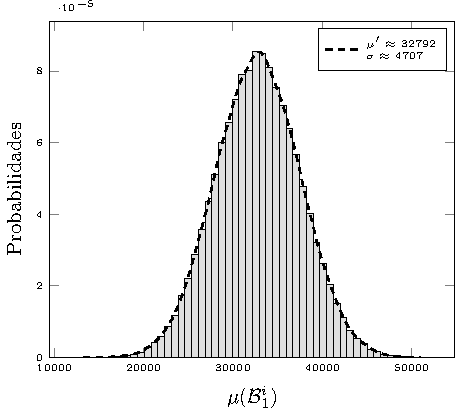
\includegraphics[width=\columnwidth]{charts/hist}
    \caption{Normalized histogram of $\mu(\mathcal{B}_{r,1})$, with $50$ bins.}
    \label{fig:dist}
\end{figure}

\begin{figure}[ht]
    \centering
    \begin{tikzpicture}
    \begin{axis}[
        axis lines = left,
        xlabel = $R$,
        ylabel = Probability,
        legend style={at={(1,0.5)},anchor=east},
    ]
    \addplot [
        domain=0:200,
        samples=100,
        thick,
        densely dashed
    ]
    {1 - (1 - 0.1587)^x};
    \addlegendentry{$P(\mu(\mathcal{B}_{r,1}) > \mu' + \sigma)$}
    \addplot [
        domain=0:200,
        samples=100,
        thick,
        loosely dashdotdotted
    ]
    {1 - (1 - 0.0228)^x};
    \addlegendentry{$P(\mu(\mathcal{B}_{r,1}) > \mu' + 2\sigma)$}
    \addplot [
        domain=0:200,
        samples=100,
        thick,
        dashdotted
    ]
    {1 - (1 - 0.0013)^x};
    \addlegendentry{$P(\mu(\mathcal{B}_{r,1}) > \mu' + 3\sigma)$}
    \end{axis}
    \end{tikzpicture}
    \label{fig:rplot}
    \caption{Thresholds for $R$.}
\end{figure}


\subsection{Security Considerations}

Our proposal makes no attempt to modify the underlying classical \textsc{Wots} mechanisms.
Hence, we discuss the impact of appending a cryptographic nonce $\lambda_r$ to a message $M$ before hashing it.
Recall that we must find a suitable hash $d_r = \mathcal{H}(M \mid\mid \lambda_r)$ such that it
produces a maximized or minimized sum of $\mathcal{B}_{r,1}$. In other words, high-order bits of 
various blocks in $\mathcal{B}_{r,1}$ have high probability of being fixed, making partial hash 
collision attacks more susceptible.

This behavior may be exploited through differential cryptanalysis on the fixed bits for the
Merkle-Damg\r{a}rd construction, recently put in practice to generate the first practical collision
for SHA-1~\cite{Stevens2017}. Such an attack could present a threat to our proposal, thus requiring the use of cryptographic hash functions which are second preimage resilient, such as SHA-256. We leave the remaining security considerations  for the scheme to be taken from~\cite{Hlsing2013}.

\section{Experiments}
\label{sec:experiments}

As a proof-of-concept, we compare the number of iterations of a function $f$ throughout
the entire execution of the digital signature schemes. Again,
we denote the four variants tested as \textsc{Wots} for the classical
scheme described on Section~\ref{sec:classical}, \textsc{Wots-b}
for the variant described on Section~\ref{sec:checksum},
\textsc{Wots-r} is the scheme described on Section~\ref{sec:counter}
and \textsc{Wots-br} merges the characteristics of the latter two.
Considering the discussion on Subsection~\ref{sub:threshold},
sufficient values of $R$ were chosen according to the usual values
of the Winternitz parameter $w$.

In Table~\ref{table:1} we give the average number of iterations
of $f$ needed to verify a signature. We experiment with $2^{14}$
executions of the verification step for the proposed schemes,
with $\mathcal{H}= $ SHA-256,
$m = 256$ and base-16 messages of $2^{10}$ length generated
through \texttt{/dev/urandom}. To better understand the effect of
each proposal individually, we also compute the average of
$\mathcal{B}_1$ and $\mathcal{B}_2$ separately. 

Note that $\mu(\mathcal{B}_2)$ is affected negatively by
\textsc{Wots-r}, since maximizing the sum of elements
in $\mathcal{B}_1$ has a direct impact on the calculation of the checksum.
However, this difference does not heavily impact the overall gains 
achieved in $\mu(\mathcal{B}_1)$. Furthermore, by using \textsc{Wots-br}, this 
behavior is greatly mitigated and may speed up the signature generation or 
verification steps up to a factor of half in a best-case scenario.

\begin{table}[htbp]
    \setlength{\tabcolsep}{7pt}
    \centering
    \caption{Number of iterations of $f$ on the verification step for
    the proposed schemes when $max(S)$ is chosen.}
    \begin{tabular}{cclccc}
    \toprule
    $w$ & $R$ & \textsc{Scheme} & $\mu(\mathcal{B}_1)$ & $\mu(\mathcal{B}_2)$ & $\mu(\mathcal{B})$ \\
    \toprule
    \multirow{8}{*}{4} & \multirow{2}{*}{-}
       &    \textsc{Wots} &     \multirow{2}{*}{479.93} &      25.88 &     505.80 \\
     & &  \textsc{Wots-b} &      &      12.25 &     492.18 \\ \cline{2-6}
    & \multirow{2}{*}{25}
       &  \textsc{Wots-r} &     \multirow{2}{*}{407.81} &      27.49 &     435.29 \\
     & & \textsc{Wots-br} &      &      13.49 &     421.29 \\ \cline{2-6}
    & \multirow{2}{*}{200}
       &  \textsc{Wots-r} &     \multirow{2}{*}{379.08} &      29.23 &     408.31 \\
     & & \textsc{Wots-br} &      &      15.23 &     394.31 \\ \cline{2-6}
    & \multirow{2}{*}{3500}
       &  \textsc{Wots-r} &     \multirow{2}{*}{348.88} &      31.14 &     380.02 \\
     & & \textsc{Wots-br} &      &      17.14 &     366.02 \\ \hline
    \multirow{8}{*}{8} & \multirow{2}{*}{-}
       &    \textsc{Wots} &    \multirow{2}{*}{4081.84} &     368.43 &    4450.27 \\
     & &  \textsc{Wots-b} &      &     136.25 &    4218.08 \\ \cline{2-6}
    & \multirow{2}{*}{25}
       &  \textsc{Wots-r} &    \multirow{2}{*}{3262.39} &     370.56 &    3632.95 \\
     & & \textsc{Wots-br} &      &     130.56 &    3392.95 \\ \cline{2-6}
    & \multirow{2}{*}{200}
       &  \textsc{Wots-r} &    \multirow{2}{*}{2940.63} &     372.13 &    3312.76 \\
     & & \textsc{Wots-br} &      &     132.13 &    3072.76 \\ \cline{2-6}
    & \multirow{2}{*}{3500}
       &  \textsc{Wots-r} &    \multirow{2}{*}{2604.49} &     374.75 &    2979.24 \\
     & & \textsc{Wots-br} &      &     134.75 &    2739.24 \\ \hline
    \multirow{8}{*}{16} & \multirow{2}{*}{-}
       &    \textsc{Wots} &  \multirow{2}{*}{525120.63} &   98231.81 &  623352.44 \\
     & &  \textsc{Wots-b} &      &   32707.82 &  557828.45 \\ \cline{2-6}
    & \multirow{2}{*}{25}
       &  \textsc{Wots-r} &  \multirow{2}{*}{376550.24} &   98225.54 &  474775.78 \\
     & & \textsc{Wots-br} &      &   32697.52 &  409247.76 \\ \cline{2-6}
    & \multirow{2}{*}{200}
       &  \textsc{Wots-r} &  \multirow{2}{*}{319490.02} &   98850.06 &  418340.08 \\
     & & \textsc{Wots-br} &      &   33321.91 &  352811.94 \\ \cline{2-6}
    & \multirow{2}{*}{3500}
       &  \textsc{Wots-r} &  \multirow{2}{*}{262301.92} &  101022.36 &  363324.28 \\
     & & \textsc{Wots-br} &      &   35492.57 &  297794.48 \\
    \bottomrule
    \end{tabular}
    \label{table:1}
\end{table}

In general, we observe a reduction of roughly $2^w$ iterations of $f$ with \textsc{Wots-b} alone. In the case of \textsc{Wots-r}, we obtain a reduction of up to $25\%$ for $w = 4$, $33\%$ for $w = 8$ and $42\%$ for $w = 16$. By merging both schemes together, we improve these results to $28\%, 39\%\text{ and }52\%$, respectively.

The aforementioned reductions translate to an increase of similar magnitude on the signature generation. For example, according to Section~\ref{sec:classical} and by letting $w = 4$, then $t = 67$ and the total number of iterations of $f$ for signature generation and verification is equal to $t \times 2^w = 1072$. Our results show that, when $R = 25$ with \textsc{Wots-br}, we can decrease the number of iterations of $f$ during the signature verification from approximately $506$ to $421$, in average.

Avoiding these $85$ iterations of $f$ during the signature verification means that we must now calculate these on the signature generation. In other words, this amounts to a $16.8\%$ speedup for the verification step at the cost of a $15\%$ slowdown during the signature generation, without taking the computation of $R$ into account.

We can substantially increase this trade-off by letting $R = 200$ or $R = 3500$, when signature generation time is not constrained. Otherwise, for small values of $w$, the number of hashes used for \textsc{Wots-r} might not be an attractive choice. Hence, such values can be better used with greater values of $w$, where computing hundreds of hash functions is negligible compared to $t \times 2^w$.

\subsection{Impact on Merkle signature schemes}

Our proposal has significant results for hash-based schemes that make
use of Merkle tree structures. We test \textsc{Wots-b}, \textsc{Wots-r} and \textsc{Wots-br} with the public
domain\footnote{\texttt{\url{https://github.com/joostrijneveld/xmss-reference/}}} reference
implementation of \textsc{Xmss} for the IETF Internet Draft
\cite{irtf-cfrg-xmss-hash-based-signatures-12}. 

We patch the reference implementation by modifying the padding process inside the \textsc{Wots+} signing algorithm, according to Section~\ref{sec:checksum}, denoting this modification as \textsc{Xmss-b}. Furthermore, by choosing $R$ with the method described in Section~\ref{sec:counter}, we achieve up to $32\%$ of speedup when benchmarking the verification step for \textsc{Xmss}. We call this variant \textsc{Xmss-r}. Additionally, when these optimizations are used together, we call the resulting scheme \textsc{Xmss-br}. 

Table~\ref{table:2} shows the average run time of $2^{14}$ signatures for each scheme, including the computation of $R$ for \textsc{Xmss-r}. We use the recommended value of $w = 4$, and additionally, $w = 8$. For greater values of $w$ (e.g. $16$), it is widely known that the \textsc{Xmss} key generation algorithm is too slow and unpractical. Hence, this value is omitted from the results. Furthermore, we experiment with both $max(S)$ and $min(S)$ to demonstrate the impact of our schemes when choosing to optimize signature verification or generation, respectively. In the case of $min(S)$, \textsc{Xmss-b} and \textsc{Xmss-br} are not considered, since \textsc{Wots}' default padding already optimizes signature generation.

\begin{table}[htbp]
    \setlength{\tabcolsep}{8pt}
    \centering
    \caption{Signature generation and verification run times (in ms)
    for the proposed schemes.}
    \begin{tabular}{ccclcc}
    \toprule
    & $w$ & $R$ & \textsc{Scheme} & \textsc{Sig. time} & \textsc{Ver. time} \\
    \toprule
    \multirow{16}{*}{\rotatebox[origin=c]{90}{$max(S)$}}
    & \multirow{8}{*}{4} & \multirow{2}{*}{-}  
    &    \textsc{Xmss}                  & 0.953  & 0.734 \\
    &&&  \textsc{Xmss-b}                & 0.975  & 0.724 \\ 
    \cline{3-6} && \multirow{2}{*}{25}   
    &   \textsc{Xmss-r}                 & 1.059  & 0.652 \\
    &&& \textsc{Xmss-br}                & 1.073  & 0.637 \\ 
    \cline{3-6} && \multirow{2}{*}{200}  
    &   \textsc{Xmss-r}                 & 1.222  & 0.620 \\
    &&&  \textsc{Xmss-br}               & 1.240  & 0.616 \\ 
    \cline{3-6} && \multirow{2}{*}{3500} 
    &   \textsc{Xmss-r}                 & 3.724  & 0.588 \\
    &&& \textsc{Xmss-br}                & 3.730  & 0.573 \\ 
    \cline{2-6} & \multirow{8}{*}{8} & \multirow{2}{*}{-} 
    &   \textsc{Xmss}                   & 7.709  & 5.676 \\
    &&& \textsc{Xmss-b}                 & 7.908  & 5.361 \\ 
    \cline{3-6} && \multirow{2}{*}{25} 
    & \textsc{Xmss-r}                   & 8.597  & 4.637 \\
    &&&  \textsc{Xmss-br}               & 8.992  & 4.415 \\ 
    \cline{3-6} && \multirow{2}{*}{200} 
    &   \textsc{Xmss-r}                 & 9.045  & 4.245 \\
    &&& \textsc{Xmss-br}                & 9.460  & 4.052 \\ 
    \cline{3-6} && \multirow{2}{*}{3500} 
    &   \textsc{Xmss-r}                 & 11.760 & 3.861 \\
    &&& \textsc{Xmss-br}                & 12.193 & 3.664 \\
    \midrule
    \multirow{8}{*}{\rotatebox[origin=c]{90}{$min(S)$}}
    & \multirow{4}{*}{4} & -
    &    \textsc{Xmss}                  & 0.971 & 0.746 \\
    && 25
    & \multirow{3}{*}{\textsc{Xmss-r}}  & 0.879 & 0.832 \\
    && 200  
    &                                   & 1.006 & 0.885 \\
    && 3500
    &                                   & 3.393 & 0.898 \\
    \cline{2-6} & \multirow{4}{*}{8} & - 
    &   \textsc{Xmss}                   & 7.819 & 5.731 \\
    && 25 
    & \multirow{3}{*}{\textsc{Xmss-r}}  & 6.672 & 6.553 \\
    && 200
    &                                   & 6.472 & 6.982 \\
    && 3500
    &                                   & 8.488 & 7.435 \\
    \bottomrule
    \end{tabular}
    \label{table:2}
    \medskip
    
    Relevant computer specifications are as follows:
    8 GB of DDR3 RAM @ 1333MHz, Intel Core i5-4570 @ 3.2GHz
    and \texttt{gcc} 7.3.0. Base commit for the modifications:
    05dac989c40349ad5f4dfee3b563b85131b95332.
\end{table}

Our results in Table~\ref{table:2} show that, for $max(S)$, any value of $R$ improves the signature verification run time, with the associated cost on signature generation. Evidently, this behavior is suppressed with greater values of $w$. However, for $min(S)$, not every value of $R$ may be chosen. In the case of $w = 4$ and $R = 25$, we obtain a speedup of $9.4\%$ for the signature generation process, while when $R = 200$ or $R = 3500$, both processes present a slower run time. The same reasoning applies to $w = 8$, where one should only choose $R = 25$ or $R = 200$.

\section{Final Remarks}

In this paper, we propose methods to adjust \textsc{Wots} for faster signature verification at the cost of a slower signature generation, or vice-versa. Our first proposal, \textsc{Wots-b}, consists of flipping the checksum padding bits, thus improving signature verification run time. In our second proposal, \textsc{Wots-r}, we present a choice to to maximize or minimize the base-$w$ blocks constructed from the message digest. The former is used to speed up signature verification, whereas the latter speeds up signature generation or verification.

We experiment with the classical Winternitz scheme and a state-of-the-art Merkle-based signature scheme, \textsc{Xmss}. We obtain an improvement factor of up to two when $w = 16$, for the \textsc{Wots} signature verification process, with regards to the number of iterations of $f$. Also, by applying our proposals to \textsc{Xmss}, we reduce the run time for the verification step by $22\%$ when $w = 4$ and $36\%$ when $w = 8$. Finally, when improving signature generation, for $w = 4$ and $w = 8$, we obtain speedups of $9.4\%$ and $17.2\%$, respectively.

\subsection{Future Works}
Throughout our work, we consider using $min(S)$ and $max(S)$ to find cryptographic nonces that speed up the \textsc{Wots} scheme. However, this may not be the best approach. We believe that the criteria for choosing $\lambda_r$ can be improved, by searching for $\mathcal{B}_{r,1}$ with elements of similar magnitude, in addition to the original proposal of $\mu(\mathcal{B}_{r,1}) > \mu'$. Parallel implementations can exploit this trait and allow faster computations of $f$.

\chapter{Conclusão}

\section{Trabalhos futuros}

\bibliographystyle{apalike}
\bibliography{ref}

\end{document}
